% Options for packages loaded elsewhere
\PassOptionsToPackage{unicode}{hyperref}
\PassOptionsToPackage{hyphens}{url}
\PassOptionsToPackage{dvipsnames,svgnames,x11names}{xcolor}
%
\documentclass[
  letterpaper,
  DIV=11,
  numbers=noendperiod,
  oneside]{scrreprt}

\usepackage{amsmath,amssymb}
\usepackage{iftex}
\ifPDFTeX
  \usepackage[T1]{fontenc}
  \usepackage[utf8]{inputenc}
  \usepackage{textcomp} % provide euro and other symbols
\else % if luatex or xetex
  \usepackage{unicode-math}
  \defaultfontfeatures{Scale=MatchLowercase}
  \defaultfontfeatures[\rmfamily]{Ligatures=TeX,Scale=1}
\fi
\usepackage{lmodern}
\ifPDFTeX\else  
    % xetex/luatex font selection
\fi
% Use upquote if available, for straight quotes in verbatim environments
\IfFileExists{upquote.sty}{\usepackage{upquote}}{}
\IfFileExists{microtype.sty}{% use microtype if available
  \usepackage[]{microtype}
  \UseMicrotypeSet[protrusion]{basicmath} % disable protrusion for tt fonts
}{}
\makeatletter
\@ifundefined{KOMAClassName}{% if non-KOMA class
  \IfFileExists{parskip.sty}{%
    \usepackage{parskip}
  }{% else
    \setlength{\parindent}{0pt}
    \setlength{\parskip}{6pt plus 2pt minus 1pt}}
}{% if KOMA class
  \KOMAoptions{parskip=half}}
\makeatother
\usepackage{xcolor}
\usepackage[left=1in,marginparwidth=2.0666666666667in,textwidth=4.1333333333333in,marginparsep=0.3in]{geometry}
\setlength{\emergencystretch}{3em} % prevent overfull lines
\setcounter{secnumdepth}{5}
% Make \paragraph and \subparagraph free-standing
\makeatletter
\ifx\paragraph\undefined\else
  \let\oldparagraph\paragraph
  \renewcommand{\paragraph}{
    \@ifstar
      \xxxParagraphStar
      \xxxParagraphNoStar
  }
  \newcommand{\xxxParagraphStar}[1]{\oldparagraph*{#1}\mbox{}}
  \newcommand{\xxxParagraphNoStar}[1]{\oldparagraph{#1}\mbox{}}
\fi
\ifx\subparagraph\undefined\else
  \let\oldsubparagraph\subparagraph
  \renewcommand{\subparagraph}{
    \@ifstar
      \xxxSubParagraphStar
      \xxxSubParagraphNoStar
  }
  \newcommand{\xxxSubParagraphStar}[1]{\oldsubparagraph*{#1}\mbox{}}
  \newcommand{\xxxSubParagraphNoStar}[1]{\oldsubparagraph{#1}\mbox{}}
\fi
\makeatother

\usepackage{color}
\usepackage{fancyvrb}
\newcommand{\VerbBar}{|}
\newcommand{\VERB}{\Verb[commandchars=\\\{\}]}
\DefineVerbatimEnvironment{Highlighting}{Verbatim}{commandchars=\\\{\}}
% Add ',fontsize=\small' for more characters per line
\usepackage{framed}
\definecolor{shadecolor}{RGB}{241,243,245}
\newenvironment{Shaded}{\begin{snugshade}}{\end{snugshade}}
\newcommand{\AlertTok}[1]{\textcolor[rgb]{0.68,0.00,0.00}{#1}}
\newcommand{\AnnotationTok}[1]{\textcolor[rgb]{0.37,0.37,0.37}{#1}}
\newcommand{\AttributeTok}[1]{\textcolor[rgb]{0.40,0.45,0.13}{#1}}
\newcommand{\BaseNTok}[1]{\textcolor[rgb]{0.68,0.00,0.00}{#1}}
\newcommand{\BuiltInTok}[1]{\textcolor[rgb]{0.00,0.23,0.31}{#1}}
\newcommand{\CharTok}[1]{\textcolor[rgb]{0.13,0.47,0.30}{#1}}
\newcommand{\CommentTok}[1]{\textcolor[rgb]{0.37,0.37,0.37}{#1}}
\newcommand{\CommentVarTok}[1]{\textcolor[rgb]{0.37,0.37,0.37}{\textit{#1}}}
\newcommand{\ConstantTok}[1]{\textcolor[rgb]{0.56,0.35,0.01}{#1}}
\newcommand{\ControlFlowTok}[1]{\textcolor[rgb]{0.00,0.23,0.31}{\textbf{#1}}}
\newcommand{\DataTypeTok}[1]{\textcolor[rgb]{0.68,0.00,0.00}{#1}}
\newcommand{\DecValTok}[1]{\textcolor[rgb]{0.68,0.00,0.00}{#1}}
\newcommand{\DocumentationTok}[1]{\textcolor[rgb]{0.37,0.37,0.37}{\textit{#1}}}
\newcommand{\ErrorTok}[1]{\textcolor[rgb]{0.68,0.00,0.00}{#1}}
\newcommand{\ExtensionTok}[1]{\textcolor[rgb]{0.00,0.23,0.31}{#1}}
\newcommand{\FloatTok}[1]{\textcolor[rgb]{0.68,0.00,0.00}{#1}}
\newcommand{\FunctionTok}[1]{\textcolor[rgb]{0.28,0.35,0.67}{#1}}
\newcommand{\ImportTok}[1]{\textcolor[rgb]{0.00,0.46,0.62}{#1}}
\newcommand{\InformationTok}[1]{\textcolor[rgb]{0.37,0.37,0.37}{#1}}
\newcommand{\KeywordTok}[1]{\textcolor[rgb]{0.00,0.23,0.31}{\textbf{#1}}}
\newcommand{\NormalTok}[1]{\textcolor[rgb]{0.00,0.23,0.31}{#1}}
\newcommand{\OperatorTok}[1]{\textcolor[rgb]{0.37,0.37,0.37}{#1}}
\newcommand{\OtherTok}[1]{\textcolor[rgb]{0.00,0.23,0.31}{#1}}
\newcommand{\PreprocessorTok}[1]{\textcolor[rgb]{0.68,0.00,0.00}{#1}}
\newcommand{\RegionMarkerTok}[1]{\textcolor[rgb]{0.00,0.23,0.31}{#1}}
\newcommand{\SpecialCharTok}[1]{\textcolor[rgb]{0.37,0.37,0.37}{#1}}
\newcommand{\SpecialStringTok}[1]{\textcolor[rgb]{0.13,0.47,0.30}{#1}}
\newcommand{\StringTok}[1]{\textcolor[rgb]{0.13,0.47,0.30}{#1}}
\newcommand{\VariableTok}[1]{\textcolor[rgb]{0.07,0.07,0.07}{#1}}
\newcommand{\VerbatimStringTok}[1]{\textcolor[rgb]{0.13,0.47,0.30}{#1}}
\newcommand{\WarningTok}[1]{\textcolor[rgb]{0.37,0.37,0.37}{\textit{#1}}}

\providecommand{\tightlist}{%
  \setlength{\itemsep}{0pt}\setlength{\parskip}{0pt}}\usepackage{longtable,booktabs,array}
\usepackage{calc} % for calculating minipage widths
% Correct order of tables after \paragraph or \subparagraph
\usepackage{etoolbox}
\makeatletter
\patchcmd\longtable{\par}{\if@noskipsec\mbox{}\fi\par}{}{}
\makeatother
% Allow footnotes in longtable head/foot
\IfFileExists{footnotehyper.sty}{\usepackage{footnotehyper}}{\usepackage{footnote}}
\makesavenoteenv{longtable}
\usepackage{graphicx}
\makeatletter
\newsavebox\pandoc@box
\newcommand*\pandocbounded[1]{% scales image to fit in text height/width
  \sbox\pandoc@box{#1}%
  \Gscale@div\@tempa{\textheight}{\dimexpr\ht\pandoc@box+\dp\pandoc@box\relax}%
  \Gscale@div\@tempb{\linewidth}{\wd\pandoc@box}%
  \ifdim\@tempb\p@<\@tempa\p@\let\@tempa\@tempb\fi% select the smaller of both
  \ifdim\@tempa\p@<\p@\scalebox{\@tempa}{\usebox\pandoc@box}%
  \else\usebox{\pandoc@box}%
  \fi%
}
% Set default figure placement to htbp
\def\fps@figure{htbp}
\makeatother
% definitions for citeproc citations
\NewDocumentCommand\citeproctext{}{}
\NewDocumentCommand\citeproc{mm}{%
  \begingroup\def\citeproctext{#2}\cite{#1}\endgroup}
\makeatletter
 % allow citations to break across lines
 \let\@cite@ofmt\@firstofone
 % avoid brackets around text for \cite:
 \def\@biblabel#1{}
 \def\@cite#1#2{{#1\if@tempswa , #2\fi}}
\makeatother
\newlength{\cslhangindent}
\setlength{\cslhangindent}{1.5em}
\newlength{\csllabelwidth}
\setlength{\csllabelwidth}{3em}
\newenvironment{CSLReferences}[2] % #1 hanging-indent, #2 entry-spacing
 {\begin{list}{}{%
  \setlength{\itemindent}{0pt}
  \setlength{\leftmargin}{0pt}
  \setlength{\parsep}{0pt}
  % turn on hanging indent if param 1 is 1
  \ifodd #1
   \setlength{\leftmargin}{\cslhangindent}
   \setlength{\itemindent}{-1\cslhangindent}
  \fi
  % set entry spacing
  \setlength{\itemsep}{#2\baselineskip}}}
 {\end{list}}
\usepackage{calc}
\newcommand{\CSLBlock}[1]{\hfill\break\parbox[t]{\linewidth}{\strut\ignorespaces#1\strut}}
\newcommand{\CSLLeftMargin}[1]{\parbox[t]{\csllabelwidth}{\strut#1\strut}}
\newcommand{\CSLRightInline}[1]{\parbox[t]{\linewidth - \csllabelwidth}{\strut#1\strut}}
\newcommand{\CSLIndent}[1]{\hspace{\cslhangindent}#1}

\KOMAoption{captions}{tableheading}
\makeatletter
\@ifpackageloaded{tcolorbox}{}{\usepackage[skins,breakable]{tcolorbox}}
\@ifpackageloaded{fontawesome5}{}{\usepackage{fontawesome5}}
\definecolor{quarto-callout-color}{HTML}{909090}
\definecolor{quarto-callout-note-color}{HTML}{0758E5}
\definecolor{quarto-callout-important-color}{HTML}{CC1914}
\definecolor{quarto-callout-warning-color}{HTML}{EB9113}
\definecolor{quarto-callout-tip-color}{HTML}{00A047}
\definecolor{quarto-callout-caution-color}{HTML}{FC5300}
\definecolor{quarto-callout-color-frame}{HTML}{acacac}
\definecolor{quarto-callout-note-color-frame}{HTML}{4582ec}
\definecolor{quarto-callout-important-color-frame}{HTML}{d9534f}
\definecolor{quarto-callout-warning-color-frame}{HTML}{f0ad4e}
\definecolor{quarto-callout-tip-color-frame}{HTML}{02b875}
\definecolor{quarto-callout-caution-color-frame}{HTML}{fd7e14}
\makeatother
\makeatletter
\@ifpackageloaded{bookmark}{}{\usepackage{bookmark}}
\makeatother
\makeatletter
\@ifpackageloaded{caption}{}{\usepackage{caption}}
\AtBeginDocument{%
\ifdefined\contentsname
  \renewcommand*\contentsname{Table of contents}
\else
  \newcommand\contentsname{Table of contents}
\fi
\ifdefined\listfigurename
  \renewcommand*\listfigurename{List of Figures}
\else
  \newcommand\listfigurename{List of Figures}
\fi
\ifdefined\listtablename
  \renewcommand*\listtablename{List of Tables}
\else
  \newcommand\listtablename{List of Tables}
\fi
\ifdefined\figurename
  \renewcommand*\figurename{Figure}
\else
  \newcommand\figurename{Figure}
\fi
\ifdefined\tablename
  \renewcommand*\tablename{Table}
\else
  \newcommand\tablename{Table}
\fi
}
\@ifpackageloaded{float}{}{\usepackage{float}}
\floatstyle{ruled}
\@ifundefined{c@chapter}{\newfloat{codelisting}{h}{lop}}{\newfloat{codelisting}{h}{lop}[chapter]}
\floatname{codelisting}{Listing}
\newcommand*\listoflistings{\listof{codelisting}{List of Listings}}
\makeatother
\makeatletter
\makeatother
\makeatletter
\@ifpackageloaded{caption}{}{\usepackage{caption}}
\@ifpackageloaded{subcaption}{}{\usepackage{subcaption}}
\makeatother
\makeatletter
\@ifpackageloaded{sidenotes}{}{\usepackage{sidenotes}}
\@ifpackageloaded{marginnote}{}{\usepackage{marginnote}}
\makeatother

\usepackage{bookmark}

\IfFileExists{xurl.sty}{\usepackage{xurl}}{} % add URL line breaks if available
\urlstyle{same} % disable monospaced font for URLs
\hypersetup{
  pdftitle={STA2020 ANOVA Notes},
  pdfauthor={Ané Cloete},
  colorlinks=true,
  linkcolor={blue},
  filecolor={Maroon},
  citecolor={Blue},
  urlcolor={Blue},
  pdfcreator={LaTeX via pandoc}}


\title{STA2020 ANOVA Notes}
\author{Ané Cloete}
\date{2024-12-17}

\begin{document}
\maketitle

\renewcommand*\contentsname{Table of contents}
{
\hypersetup{linkcolor=}
\setcounter{tocdepth}{2}
\tableofcontents
}

\bookmarksetup{startatroot}

\chapter*{Preface}\label{preface}
\addcontentsline{toc}{chapter}{Preface}

\markboth{Preface}{Preface}

This book is not an exhaustive guide for designing an experiment or
conducting ANOVA's, it has been tailored specifically for the learning
outcomes and methods covered in STA2020. If you are interested in a more
general text on experimental design, please see:

Instructions:

\begin{itemize}
\tightlist
\item
  Examples
\item
  R code
\item
  Tips
\item
  Footnotes
\end{itemize}

\bookmarksetup{startatroot}

\chapter*{Statistical Modelling}\label{statistical-modelling}
\addcontentsline{toc}{chapter}{Statistical Modelling}

\markboth{Statistical Modelling}{Statistical Modelling}

\section*{What is a Model?}\label{what-is-a-model}
\addcontentsline{toc}{section}{What is a Model?}

\markright{What is a Model?}

A \textbf{statistical model} is a mathematical representation of how
data is generated. It describes the relationship between observed data
and underlying factors (parameters) while accounting for random
variation. Suppose that we are interested in estimating the age of a
tree from its stem diameter. To do this we need to know by how much the
stem diameter increases per year. We could describe this relationship or
process as follows:

\[D = \alpha + \beta \times Age\] describing a linear increase of
diameter with age. Once we have a good idea of how fast diameter
increases with age (β) we can predict diameter from age. The
(mathematical) model above is a very simple representation of this
process with only two parameters, the intercept and the growth rate.

With the chosen parameter values, diameter increases linearly with age.
Of course, this model is not realistic except for special situations but
it gives us powerful insights. In reality we don't know \(\beta\), but
usually need to estimate it from data. Also, not every tree grows
equally fast, because of environmental and individual differences
between trees. We can accept that the above is a simple model for the
average behaviour of a tree, but to capture variability between trees
(because of variability between environmental conditions from tree to
tree, variability between individual trees, measurement error), we add
an error term.

\[D = \alpha + \beta \times Age_i + e_i\]

The response that we observe is then described by an average behaviour,
but the actual observed value will vary around this average. To
summarise, the statistical model has a stochastic component which
captures variability in the response that cannot be explained by the
deterministic part of the model. Another distinguishing feature of
statistical modelling is that we obtain estimates of the parameter
values from the data, e.g.~by fitting a line to the observations,
i.e.~we learn from data.

\section*{More generally}\label{more-generally}
\addcontentsline{toc}{section}{More generally}

\markright{More generally}

Statistical models are not perfect predictors of the data, rather they
attempt to describe the ``central tendency'' of the observations. To get
to the actual observed value some deviation from the central tendency
needs to added (i.e.~error). Such models typically have the following
the form:

\[
\text{Observed Response} = \text{Model Predicted Response} + \text{Error}
\] Mathematically this can be stated as:

\[ Y = \hat{Y} + e\]

A simple example of a statistical model you may have encountered is the
\textbf{mean} as a predictor. Suppose you measure the number of
customers entering two stores over 20 days. The observed counts for each
store fluctuate daily, but you may want to summarize the data using the
average number of customers.

For each store \(i\), a basic statistical model for these observations
would be:

\[
Y_{ij} = \mu_i + e_{ij}
\]

where:

\begin{itemize}
\tightlist
\item
  \(Y_{ij}\) is the number of customers observed on day \(j\) at store
  1,
\item
  \(\mu_i\) is the true mean number of customers at store \(i\),
\item
  \(e_{ij}\) is the error term, representing deviations from the mean.
\end{itemize}

The error term \(e_{ij}\) accounts for day-to-day fluctuations that
cause the actual number of customers to vary around the mean. Below this
data is simulated and plotted, with the model overlain. The black line
is the mean and the red dashed line represents the error for one
observation, i.e.~deviation from the fitted model response, in this case
the mean.

\pandocbounded{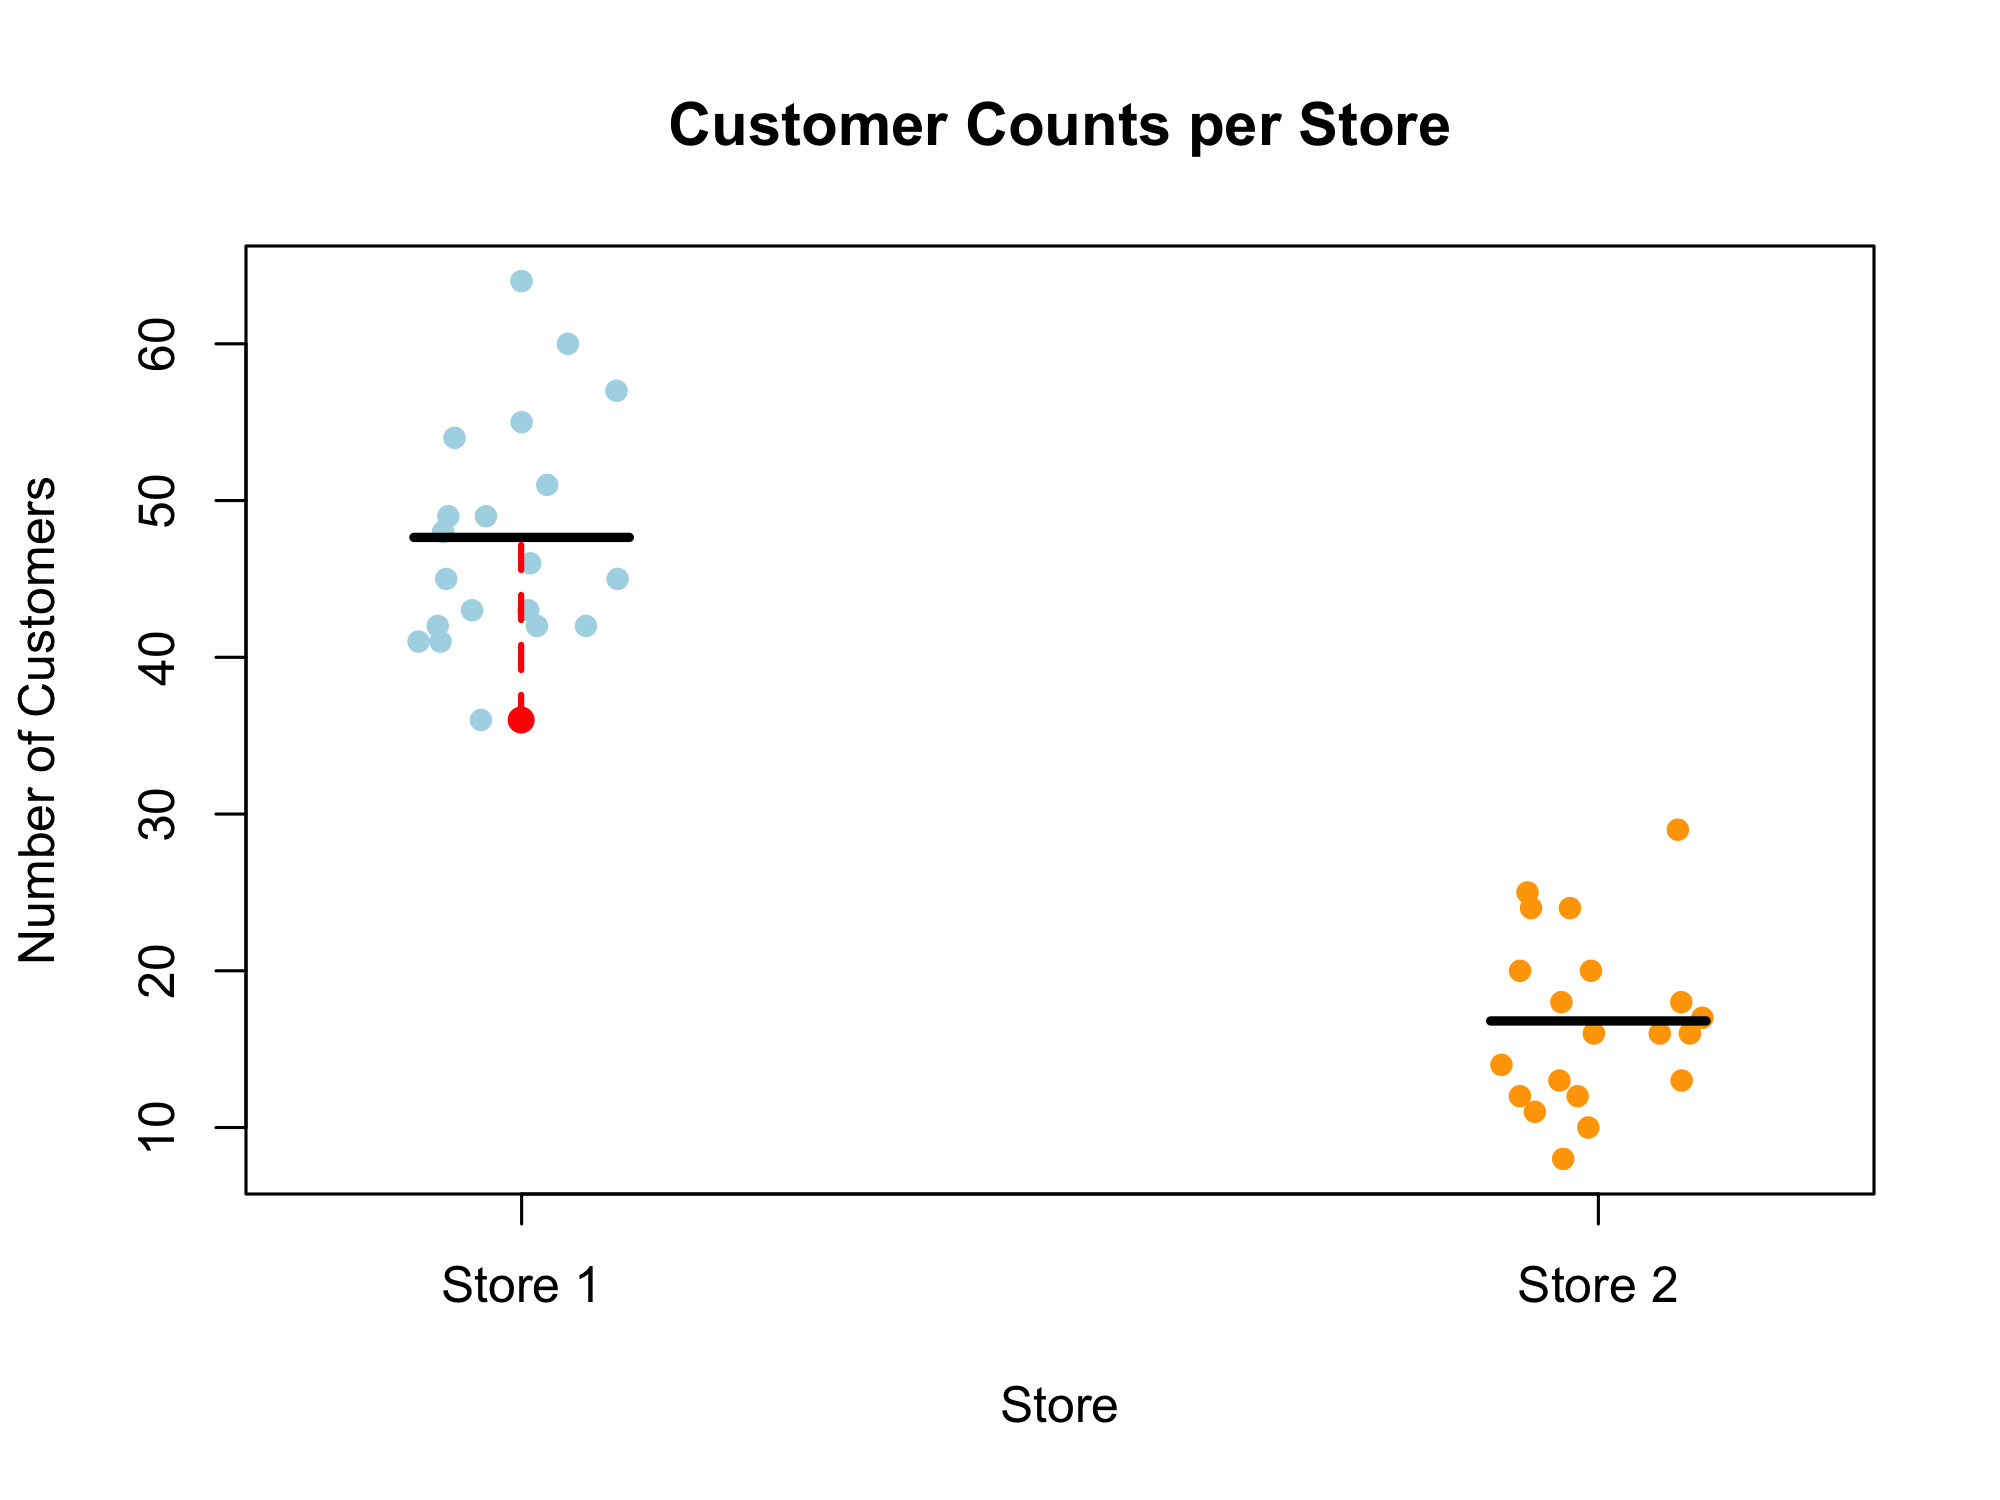
\includegraphics[keepaspectratio]{storedata2.png}}

Another basic example of this structure is a \textbf{linear regression
model}:

\[
Y_i = \beta_0 + \beta_1 X_i + e_i
\]

where:

\begin{itemize}
\tightlist
\item
  \(Y_i\) is the observed response,
\item
  \(\beta_0\) and \(\beta_1\) are unknown parameters representing the
  intercept and slope,
\item
  \(X_i\) is the predictor variable,
\item
  \(e_i\) is the random error term.
\end{itemize}

\pandocbounded{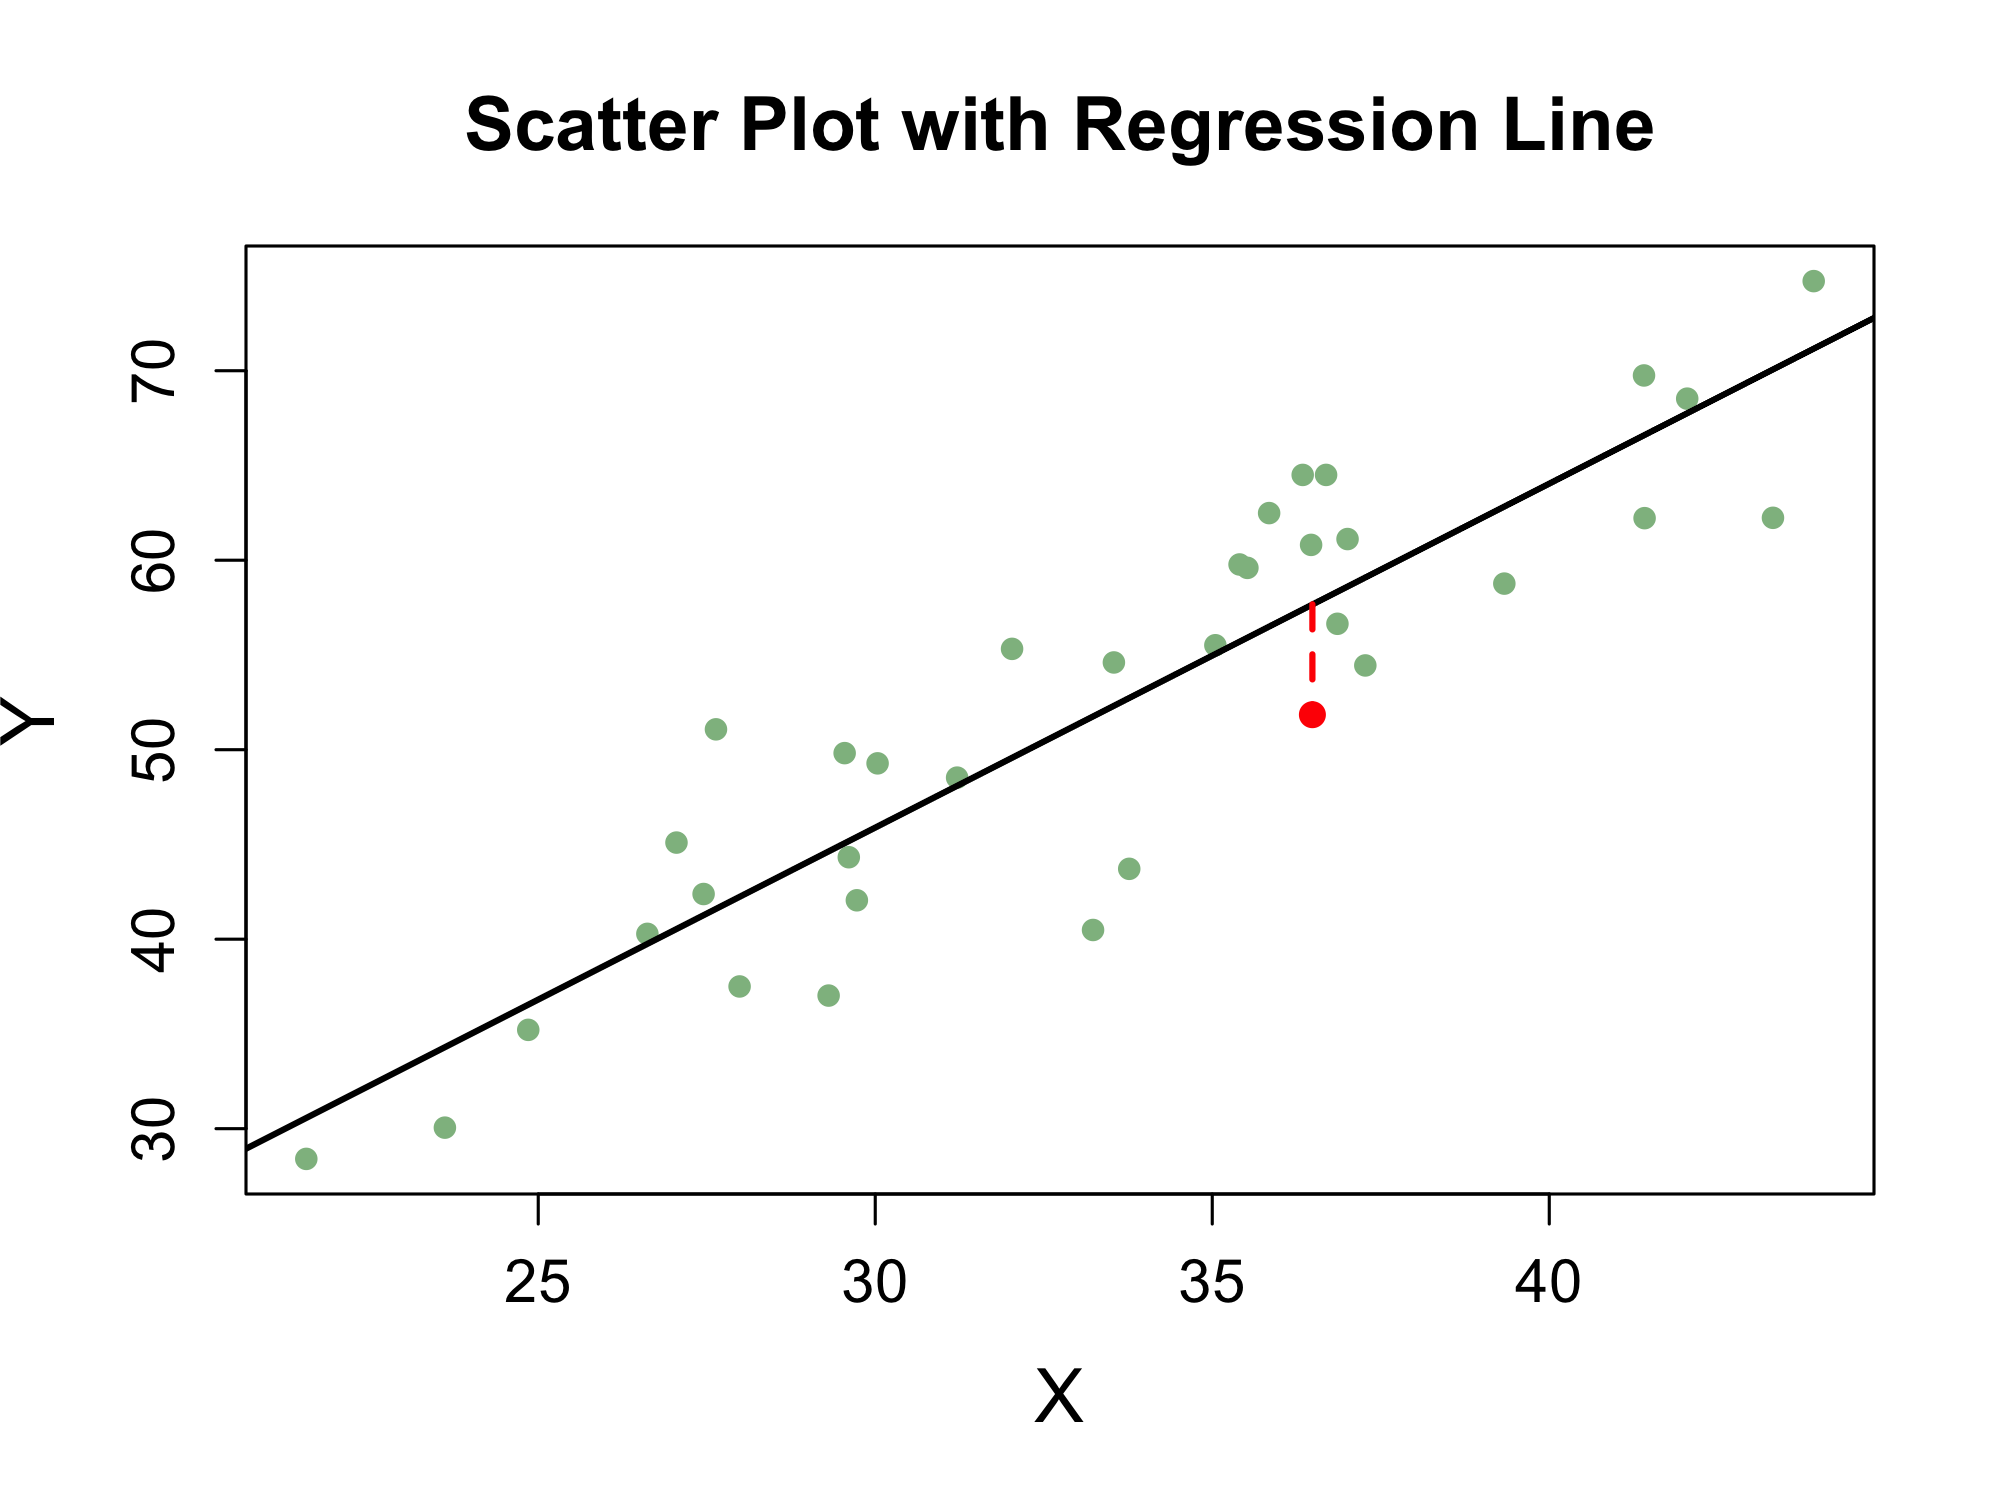
\includegraphics[keepaspectratio]{storedata3.png}}

\section*{Notation}\label{notation}
\addcontentsline{toc}{section}{Notation}

\markright{Notation}

When we fit the model to our data, we \textbf{estimate} the unknown
parameters using observed data. We denote these estimates using
\textbf{hat notation} to distinguish them from the true (but unknown)
population parameters:

\[
\hat{\beta}_0, \quad \hat{\beta}_1
\]

Similarly, the \textbf{fitted values} (model-predicted responses) are
denoted as:

\[
\hat{Y}_i = \hat{\beta}_0 + \hat{\beta}_1 X_i.
\]

Thus, after fitting the model, the observed response can be rewritten
as:

\[
Y_i = (\hat{\beta}_0 + \hat{\beta}_1 X_i) + e_i = \hat{Y}_i + e_i
\]

where:

\begin{itemize}
\tightlist
\item
  \(\hat{Y}_i\) is the \textbf{fitted (predicted) value}, and
\item
  \(e_i = Y_i - \hat{Y}_i\) is the \textbf{residual}, representing the
  difference between the observed and predicted values.
\end{itemize}

True model (unknown parameters):

\[
Y_i = \beta_0 + \beta_1 X_i + e_i
\]

and fitted model:

\[
\hat{Y}_i = \hat{\beta}_0 + \hat{\beta}_1 X_i
\]

\part{Experimental Design}

\chapter{Experiments and experimental
design}\label{experiments-and-experimental-design}

There are two fundamental ways to obtain information in research: by
\emph{observation} or by \emph{experimentation}. In an observational
study the observer watches and records information about the subject of
interest. In an experiment, the experimenter actively manipulates
variables hypothesized to affect the response (insert small example).
Although both are important ways of understanding the world around us,
only through experiments can we \textbf{infer causality}.

That is, by designing and conducting an experiment properly, if we
observe a result such as a change in variable A leads to a change in our
response (say variable B), we can conclude that A \textbf{caused} this
change in B. If we were to merely study variable B and observe that as
variable A changes, B also changes without conducting an experiment,
then we can only say that variable A and B are associated. We could not
conclude that any change in B is due to A. It could be some other factor
that is correlated with A or it could be that B caused the change in A!
The key is that a well-designed experiment controls and holds constant
(as best we can) all other factors that might affect the response, so we
can be sure the result is caused by the variable we manipulated.

Imagine a company wants to determine whether their voluntary employee
training program (the explanatory variable) increases productivity (the
response). They decide to track the productivity of employees who chose
to complete the training and those who did not. They note that, on
average, trained employees are more productive. Can we confidently
conclude that the training program caused increased productivity?

This is an observational study since no variable was actively
manipulated, they merely observed and recorded the productivity of two
groups of employees. So, we cannot conclude that completing the training
program increases productivity - we cannot infer causality. It could be
due to many other factors, either observed or unobserved, such as maybe
employees who choose to do the training program are inherently more
motivated and thus productive. Can you think of any other factors?

If they actively manipulate the explanatory variable, training program,
by randomly assigning employees to complete the training program or not
and control other factors by ensuring the employees are as similar as
possible accross the groups (i.e.~conducted an experiment). Any
differences in productivity between the two groups could then be
ascribed to the training program. If they happen to find that the
employees who were assigned the training program are more productive,
they can confidently say that the program caused increased productivity
(and perhaps make it compulsory for all employees!).

Experimental studies are extremely important in research and in
practice. They are almost the only way in which one can control all
factors to such an extent as to eliminate any other possible explanation
for a change in a response other than the variable actively manipulated.
In this course, we only consider experimental studies and those which
aim to compare the effects of a number of \textbf{treatments}.

Here are some other reasons for conducting experiments:

\begin{enumerate}
\def\labelenumi{\arabic{enumi}.}
\item
  They are easy to analyse. A well designed experiment results in
  independent estimates of treatment effects which allow us to easily
  interpret the effects. EXPAND - independent treatment effects and/or
  independent treatment variables?
\item
  Experiments are frequently used to find optimal levels of variables
  which will maximise (or minimise) the response. Such experiments can
  save enormous amounts of time and money. Imagine trying to find the
  optimal settings for producing electricity from coal without proper
  experimentation. Such a trial and error process would be extremely
  costly, wasteful and time consuming. In a similar vein, what if the
  fictional company in our previous example decided to invest a bunch of
  money in fine-tuning their training program based solely on the
  results of an observational study. In reality though, it turns out
  that adjusting their hiring process to identify more keen candidates
  would have been much more efficient and inexpensive.
\item
  In an experiment we can choose exactly those settings or
  \textbf{treatment levels} we are interested in, e.g.~we can
  investigate the effect of different shift lengths (6, 8 or 9 hours) on
  employee productivity or test specific price points (R100, R150, R200)
  to determine which price maximizes sales or revenue. We can actively
  manipulate the variable(s) to the levels we are interested in.
\end{enumerate}

Experimental studies and their design are fundamental to science,
allowing us to further knowledge and test theories. So lets define them
more rigorously. We'll start by introducing some terminology.

INSERT WHAT THEY NEED TO KNOW / MAIN TAKEAWAYS Perhaps?

\chapter{Terminology}\label{terminology}

\section*{\texorpdfstring{\textbf{Treatment factors, treatment levels
and
treatments:}}{Treatment factors, treatment levels and treatments:}}\label{treatment-factors-treatment-levels-and-treatments}
\addcontentsline{toc}{section}{\textbf{Treatment factors, treatment
levels and treatments:}}

\markright{\textbf{Treatment factors, treatment levels and treatments:}}

The \textbf{treatment factor} is the factor or variable that the
experimenter actively manipulates to measure its effect on the response.
All factors/variables that are investigated, controlled, manipulated,
thought to influence the response, are called the treatment factors.
They become the \textbf{explanatory variables} (mostly categorical) in
the model. For each treatment factor, we actively choose a set of
\textbf{levels}. For example, the treatment factor ``temperature'' can
have levels 10, 20, and 50°C. If temperature is the only treatment
factor in the experiment, the \textbf{treatments}\sidenote{\footnotesize The
  terminology of treatments can be traced back to 1920's when it was
  first applied by Ronald Fisher in the agricultural sciences. He is
  often refered to as the Founder of Statistics! Have a look at the very
  first application of ANOVA
  \href{https://www.cambridge.org/core/journals/journal-of-agricultural-science/article/abs/studies-in-crop-variation-i-an-examination-of-the-yield-of-dressed-grain-from-broadbalk/882CB236D1EC608B1A6C74CA96F82CC3}{here}
  and also a very \href{https://www.jstor.org/stable/2245989}{nice
  article} describng the history of statistics and his contribution to
  the field.} will also be 10, 20, and 50°C.

If we manipulate more than one factor (e.g., temperature and pressure),
we have two treatment factors. When several treatment factors are
manipulated, the experiment is called factorial and the
\textbf{treatments} are all possible combinations of the factor levels.
If we have pressure levels ``low'' and ``high,'' there are 6 treatments
in total:

\begin{figure}

\centering{

\pandocbounded{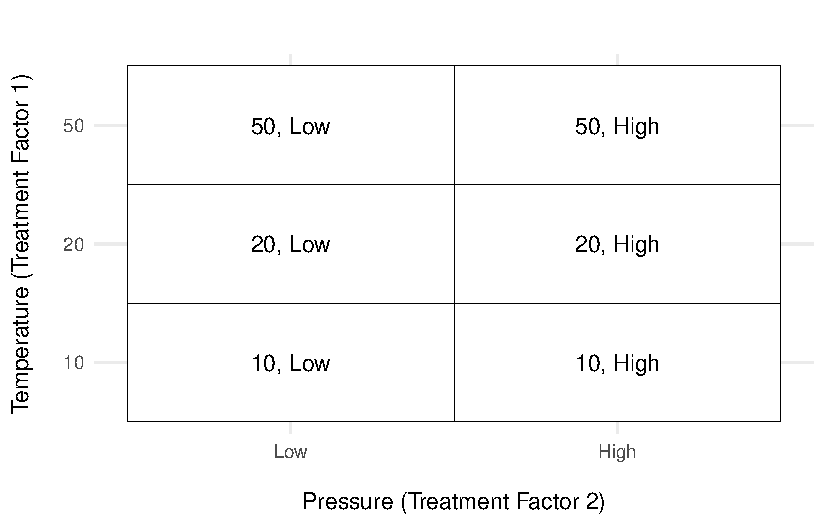
\includegraphics[keepaspectratio]{02_ExpDesign_Term_files/figure-pdf/fig-vistreat-1.pdf}}

}

\caption{\label{fig-vistreat}Visualization of how treatments are formed
as combinations of treatment levels.}

\end{figure}%

In the figure above, there are two treatment factors: Temperature (on
the y-axis) and Pressure (on the x-axis). The axis ticks represent the
levels of each treatment factor, and the blocks within the grid
represent the treatments, which are specific combinations of the levels
of Temperature and Pressure. Each treatment is labeled with the
corresponding combination of levels (e.g., `50, Low' or `10, High').

\begin{tcolorbox}[enhanced jigsaw, colframe=quarto-callout-warning-color-frame, breakable, arc=.35mm, toptitle=1mm, colback=white, title={Example 1}, opacityback=0, bottomrule=.15mm, opacitybacktitle=0.6, colbacktitle=quarto-callout-warning-color!10!white, toprule=.15mm, rightrule=.15mm, bottomtitle=1mm, leftrule=.75mm, titlerule=0mm, coltitle=black, left=2mm]

Three groups of students, 5 in each group, were receiving therapy for
severe test anxiety. Group 1 recieved 5 hours, group 2 received 10 hours
and group 3 received 15 hours. At the end of therapy each subject
completed an evaulation of test anxiety. Did the amount of therapy have
an effect on the level of test anxiety?

The three groups of studnets received the scores on the Test Anxiety
index (TAI) at the end of treatment shown in the table below.

\begin{longtable}[]{@{}ccc@{}}
\toprule\noalign{}
Group 1 & Group 2 & Group 3 \\
\midrule\noalign{}
\endhead
\bottomrule\noalign{}
\endlastfoot
48 & 55 & 51 \\
50 & 52 & 52 \\
53 & 53 & 50 \\
52 & 55 & 53 \\
50 & 53 & 50 \\
\end{longtable}

\hfill\break

\end{tcolorbox}

When faced with a text like this, it is useful to identify the treatment
factors, their levels and the treatments, as well the response. Clearly,
from the question, we are interested in the effect of therapy on test
anxiety. A statement like this can generally be read as the effect of
the treatment factor on the response. Nowhere is another treatment
factor mentioned, so we only have one in this example. What are the
levels of therapy we set? The levels are 5, 10 and 15 hours of therapy
and since we only have one factor these are also the treatments. Let's
summarise this as follows:

\begin{itemize}
\tightlist
\item
  \textbf{Response:} Test Anxiety\\
\item
  \textbf{Treatment Factor:} Therapy\\
\item
  \textbf{Treatment Levels:} 5, 10, and 15 hours of therapy\\
\item
  \textbf{Treatments:} 5, 10, and 15
\end{itemize}

\section*{\texorpdfstring{\textbf{Experimental and observational
unit}}{Experimental and observational unit}}\label{experimental-and-observational-unit}
\addcontentsline{toc}{section}{\textbf{Experimental and observational
unit}}

\markright{\textbf{Experimental and observational unit}}

The \textbf{experimental unit} is the entity (e.g.~material, object, or
individual) to which a treatment is assigned or that receives the
treatment. By contrast, the \textbf{observational unit} is the entity
from which the response is recorded. This distinction is very important
because it is the experimental units which determine how often the
treatment has been replicated and therefore the precision with which we
can measure the treatment effect. In the methods that we cover in this
course, we require that in the end there is only one `observation'
(response value) per experimental unit. If several measurements have
been taken on an experimental unit, we will combine these into one
observation, typically by taking the mean. Very often, the experimental
unit is also the observational unit.

For See Example
(\textbf{example-box?})\marginpar{\begin{footnotesize}example-box\vspace{2mm}\par\end{footnotesize}}
for more details, what are the experiemental units? To determine this,
revisit the text of Example 1 and ask yourself: what entity received the
treatments or to what were treatments applied? Most of you, will
probably answer the students and this is correct. Each student received
the respective treatment (number of hours in therapy) assigned to their
group and so there are \(5 \times 3 = 15\) experimental units.

There is an argument to be made that it is not clear whether the
students received therapy on their own or that the groups of students
received therapy together. In that case, treatments were applied to
groups of students and so there would be three experimental units. This
will usually be clear from the text, but we'll use this scenario to
illustrate some concepts as we go.

We also need to know what the observational units are. The text states
that at the end of therapy, each student completed an evaluation to
determine their level of test anxiety. So the response, test anxiety,
was measured on the student level which means students are the
observational units. In the first scenario, the students are both the
experimental units and observational units. But this would not be the
case if groups are the experimental unit.

We also require that there is only one observation per experimental
unit, the first scenario meets this requirement. For the second
scenario, we have 5 observations per group and so we would have to take
the mean of these values to end up wth one response value per group.

Let's add to the summary assuming students are the experimental units:

\begin{itemize}
\tightlist
\item
  \textbf{Experimental unit (no):} Student (15)\\
\item
  \textbf{Observational unit (no):} Student (15)
\end{itemize}

\section*{\texorpdfstring{\textbf{Homogeneity of experimental
units}}{Homogeneity of experimental units}}\label{homogeneity-of-experimental-units}
\addcontentsline{toc}{section}{\textbf{Homogeneity of experimental
units}}

\markright{\textbf{Homogeneity of experimental units}}

When the set of experimental units are as similar as possible such that
there are no distinguishable differences between them, they are said to
be \textbf{homogeneous} (a fancy word for saying they are of the same
kind). The more homogeneous the units are, the smaller the experimental
error variance (natural variation between between observations of the
same treatments) will be. It is super important to have fairly
homogeneous units because it allows us to detect differences between
treatments more easily.

\section*{\texorpdfstring{\textbf{Blocking}}{Blocking}}\label{blocking}
\addcontentsline{toc}{section}{\textbf{Blocking}}

\markright{\textbf{Blocking}}

If the experimental units are not fairly similar but are heterogeneous
(the opposite of homogeneous), we can group them into sets of similar
units. This process is called \textbf{blocking} and the groups are
considred ``blocks''. We compare the treatments within each block as if
each block is its own mini-experiment. This way we account for the
differences between blocks and can better isolate the effect of the
treatments.

\begin{tcolorbox}[enhanced jigsaw, colframe=quarto-callout-warning-color-frame, breakable, arc=.35mm, toptitle=1mm, colback=white, title={Example 2.2 EDIT THIS STILL}, opacityback=0, bottomrule=.15mm, opacitybacktitle=0.6, colbacktitle=quarto-callout-warning-color!10!white, toprule=.15mm, rightrule=.15mm, bottomtitle=1mm, leftrule=.75mm, titlerule=0mm, coltitle=black, left=2mm]

Imagine you're testing the effectiveness of two marketing strategies (A
and B) to increase sales at a chain of coffee shops. The coffee shops
are located in different neighborhoods, where factors like income levels
might influence sales. To prevent these differences from skewing the
results, you group the coffee shops into ``blocks'' based on
neighborhood income level (e.g., low, medium, high).

Within each block, you randomly assign coffee shops to either Strategy A
or Strategy B. This approach allows you to compare the strategies while
controlling for variability caused by differences in neighborhood income
levels.

Without blocking, would you be able to confidently attribute differences
in sales to the strategies alone? Likely not, as any observed
differences could be due to neighborhood-specific factors rather than
the strategies themselves.

\end{tcolorbox}

\section*{\texorpdfstring{\textbf{Replication and
pseudoreplication}}{Replication and pseudoreplication}}\label{replication-and-pseudoreplication}
\addcontentsline{toc}{section}{\textbf{Replication and
pseudoreplication}}

\markright{\textbf{Replication and pseudoreplication}}

If a treatment is applied independently to more than one experimental
unit it is said to be \textbf{replicated}. Treatments must be
replicated! Making more than one observation on the same experimental
unit is not replication, but \emph{pseudoreplication}. Pseudoreplication
is a common fallacy (REF?). The problem is that without true
replication, we don't have an estimate of uncertainty, of how
repeatable, or how variable the result is if the same treatment were to
be applied repeatedly.

In Example 1, if experimental units were the groups and we didn't take
the average of the observations per group, we would have
pseudoreplication as each student would not be an independent replicate
of a treatment - effectively, we have only applied each treatment once.
You might notice that we then only have one true replicate per treatment
group and this is problematic. To get an estimate of uncertainty, we
would have to repeat this experiment a few more times to get more than
one proper replicate.

The first scenario, however, did not have this problem and each
treatment was replicated five times. After going through all this, we
have the following summary:

\begin{itemize}
\tightlist
\item
  \textbf{Response:} Test Anxiety\\
\item
  \textbf{Treatment Factor:} Therapy\\
\item
  \textbf{Treatment Levels:} 5, 10, and 15 hours of therapy\\
\item
  \textbf{Treatments:} 5, 10, and 15\\
\item
  \textbf{Experimental unit (no):} Student (15)\\
\item
  \textbf{Observational unit (no):} Student (15)\\
\item
  \textbf{Replicates:} 5
\end{itemize}

\begin{tcolorbox}[enhanced jigsaw, colframe=quarto-callout-tip-color-frame, breakable, arc=.35mm, toptitle=1mm, colback=white, title=\textcolor{quarto-callout-tip-color}{\faLightbulb}\hspace{0.5em}{Tip}, opacityback=0, bottomrule=.15mm, opacitybacktitle=0.6, colbacktitle=quarto-callout-tip-color!10!white, toprule=.15mm, rightrule=.15mm, bottomtitle=1mm, leftrule=.75mm, titlerule=0mm, coltitle=black, left=2mm]

Creating a summary like this, is a handy exercise for any experiment you
come across, and we'll keep doing it for every experiment in this book.
As we go along, we'll also add information about the type of experiment
that was conducted.

\end{tcolorbox}

\chapter{The three R's of experimental
design}\label{the-three-rs-of-experimental-design}

\textbf{Experimental Design} is a detailed procedure for grouping, if
blocking is necessary, experimental units and for how treatments are
assigned to the experimental units. There are three fundamental
principles, known as the `three R's of experimental design' which are at
the core of a good experiment. The following section might feel a bit
repetitive, but these concepts cannot be emphasised enough.

\section{Replication}\label{replication}

Let's define it again: replication is when each treatment is applied to
several experimental units. This ensures that the variation between two
or more units receiving the same treatment can be estimated and valid
comparisons can be made between treatments. In other words, replication
allows us to separate variation due to differences between treatments
from variation within treatments. For true replication, each treatment
should be \textbf{independently} applied to several experimental units.
If this is not the case, treatment effects become confounded with other
factors.

Confounding means that is not possible to separate the effects of two
(or more) factors on the response, i.e.~it is not possible to say which
of the two factors is responsible for any changes in the response. This
is what happened in the Example 1 when groups are the experimental
units. With only one observation per experimental unit, the effect of
therapy is confounded with the experimental unit or the effect of group
on test anxiety. The reason why this is a problem is that any difference
between the treatments could be due to any differences between the
groups and not just the number of therapy hours. The same would be true
if we only had one student per group, why? Take a moment to think about
this.

Consider the first row of the data from Example 1. It looks like the
student in group 2 scored the highest, followed by group 3 and then
group 1. So does longer therapy sessions lead to higher test anxiety?
Likely not! With only one student per treatment, we are not able to say
that any differences in the response are due to the treatments. It could
be due to any differences between the individuals. Maybe the student in
group 3 tends to score higher on anxiety tests regardless of the
treatment, or perhaps the student in group 1 was unusually calm that
day. Without replication, these individual differences could mask (or
mimic) the true effects of the treatments.

By replicating the treatments across multiple students, we can average
out these individual differences and gain a clearer picture of whether
therapy duration truly impacts test anxiety. With five students per
group, we might observe that group 1 consistently scores lower than
group 3. This consistency would provide stronger evidence that the
treatments, and not just individual variation, are responsible for the
observed differences. So by replication, we can compare within treatment
variation to variation between treatments.

\begin{longtable}[]{@{}ccc@{}}
\toprule\noalign{}
Treatment 1 & Treatment 2 & Treatment 3 \\
\midrule\noalign{}
\endhead
\bottomrule\noalign{}
\endlastfoot
48 & 55 & 51 \\
50 & 52 & 52 \\
53 & 53 & 50 \\
52 & 55 & 53 \\
50 & 53 & 50 \\
\end{longtable}

\begin{tcolorbox}[enhanced jigsaw, colframe=quarto-callout-tip-color-frame, breakable, arc=.35mm, toptitle=1mm, colback=white, title={Example 3.1}, opacityback=0, bottomrule=.15mm, opacitybacktitle=0.6, colbacktitle=quarto-callout-tip-color!10!white, toprule=.15mm, rightrule=.15mm, bottomtitle=1mm, leftrule=.75mm, titlerule=0mm, coltitle=black, left=2mm]

Maybe the co2 uptake data?

\end{tcolorbox}

\section{Randomisation}\label{randomisation}

Randomisation refers to the process of randomly assigning treatments to
experimental units such that each experimental unit has equal chance of
receiving a specific treatment. Randomisation ensures that:

\begin{enumerate}
\def\labelenumi{\arabic{enumi}.}
\item
  There is no bias on the part of the experimenter, either conscious or
  unconscious, when assigning treatments to experimental units.
\item
  No experimental unit is favored to receive a particular treatment.
\item
  Possible differences between units are equally distributed amongst
  treatments. If there are clear differences between units, then
  blocking should be performed and randomisation occurs within blocks.
  We'll talk more about this in Chapter INSERT
\item
  We can assume independence between observations.
\end{enumerate}

Randomisation is not haphazard. In statistics (and here in the context
of experimental design), randomisation has a specific meaning: namely
that each experimental unit has the same chance of being allocated any
of the treatments. This can be done using random number generators such
as with software packgaes, dice or drawing number from a hat (provided
the number have been shuffled adequately and have equal chance to be
picked).

Let's have a look at randomisation in R. Suppose we have 4 treatments
(\texttt{A}, \texttt{B}, \texttt{C}, and \texttt{D}) and 32 experimental
units. There are no differences between the units, so we don't have to
block, and we can equally split the units across the treatments, which
means we have 8 units per treatment, i.e., 8 replicates. In R, we first
create a long vector of 8 \texttt{A}s, 8 \texttt{B}s, 8 \texttt{C}s, and
8 \texttt{D}s called \texttt{all.treat}. Then shuffle the vector to
obtain a randomisation using the function \texttt{sample}.

\begin{Shaded}
\begin{Highlighting}[]
\CommentTok{\# repeat the vector A, B, C, D 8 times }
\NormalTok{all.treats }\OtherTok{\textless{}{-}} \FunctionTok{rep}\NormalTok{(}\FunctionTok{c}\NormalTok{(}\StringTok{"A"}\NormalTok{,}\StringTok{"B"}\NormalTok{,}\StringTok{"C"}\NormalTok{,}\StringTok{"D"}\NormalTok{), }\AttributeTok{times =} \DecValTok{8}\NormalTok{)}

\CommentTok{\# permutation of all.treats (sample withut replacement)}
\NormalTok{rand1 }\OtherTok{\textless{}{-}} \FunctionTok{sample}\NormalTok{(all.treats)}

\CommentTok{\# example output}
\NormalTok{rand1}
\end{Highlighting}
\end{Shaded}

\begin{verbatim}
 [1] "A" "A" "B" "A" "C" "D" "D" "D" "D" "D" "B" "C" "A" "B" "A" "C" "C" "A" "B"
[20] "A" "B" "B" "C" "B" "B" "D" "C" "D" "D" "C" "A" "C"
\end{verbatim}

Experimental unit 1 recipes the first treatment that appears as the
first element in the shuffled vector, experimental unit 2 receives the
second and so on.

Notes on randomisation?

\section{Reduction of Unexplained Variation
(Blocking)}\label{reduction-of-unexplained-variation-blocking}

Unexplained variation (or experimental error variance or within
treatment variance) is largely due to inherent differences between
experimental units. The larger this unexplained variation, the more
difficult it becomes to detect treatment differences (a treatment
signal). To minimise experimental error variance we can control
extraneous factors (i.e.~keeping all else constant) and by choosing
homogeneous experimental units. Otherwise, we can \textbf{block}
experimental units to reduce the variation.

Blocking variables are nuisance factors that might affect your response
or introduce systematic variation in the response and we are typically,
not interested in these. Often, they are factors that cannot be
randomised, e.g.~biological sex of a person, time of day, location of a
warehouse etc. We control the effect of such variables on the response
by blocking for them so that we can investigate the possible effect of a
variable that we are interested in. Usually, in a \textbf{complete
block} experiment, there are as many experimental units per block as
there are treatments, so that each treatment is applied once in every
block. Treatments are randomized to the experimental units in the
blocks. We can then compare the effects of treatments on similar
experimental units, and we can estimate the variation induced in the
response due to the differences between blocks. This variation due to
blocks can then be removed from the unexplained variation.

EXAMPLE

Blocking also offers the oopurutnity to test treatments over a wider
range of conditions, e.g.~if I only use people of one age in my
experiment (say students) I cannot generalize my results to older
people. However, if i use different age blocks I will be able to tell
whether the treatments have similar effects in all age groups or not.

Lastly, if blocking is not feasible, randomization will ensure that at
least treatments and nuisance factors are not confounded.

\begin{quote}
``Block what you can, randomize what you cannot.''

--- Box, Hunter \& Hunter (1978)
\end{quote}

\chapter{Designing an Experiment}\label{designing-an-experiment}

When planning an experiment we need to decide on:

\begin{itemize}
\tightlist
\item
  treatment factors and their levels
\item
  the response
\item
  experimental material / units
\item
  blocking factors
\item
  number of replicates
\end{itemize}

Some of these will be determined by the research question and how
experimental units are assigned to treatments are determined by the
design. The design that will be chosen for a particular experiment
depends on the \textbf{treatment structure} (determined by the research
question) and the \textbf{blocking structure} (determined by the
available experimental units).

Here are two ways the treatments can be structured:

\begin{enumerate}
\def\labelenumi{\arabic{enumi}.}
\tightlist
\item
  \textbf{Single factor}: the treatments are the levels of a single
  treatment factor.
\item
  \textbf{Factorial}: when more than one factor are of interest, then
  the experiment is said to be a factorial experiment. The treatments
  are constructed by crossing the treatment factors like we did in
  Figure~\ref{fig-vistreat} such that the treatments are all possible
  combinations of the treatment levels. For example, if factor A has
  \(a\) levels and factor B has \(b\) levels, there are \(a \times b\)
  treatments. Such an experiment would then be called an \(a \times b\)
  factorial experiment.
\end{enumerate}

The blocking structure is determined the set of experimental units
chosen or available for the experiment.are there any
structures/differences that need to be blocked? Do I want to include
experimental units of different types to make the results more general?
How many experimental units are available in each block? For the
simplest design in this course, the number of experimental units in each
block corresponds to the number of treatments. This is called a complete
block experiment. There are several other blocking structures, such as
incomplete blocks and blocks with missing values, all with specific
analysis which we will not cover here.

In this course, we cover two basic designs: Completely Randomized
Designs (CRD) and Randomized Block Designs (RBD). For both designs, the
treatment structure can be single or factorial. Where they differ is in
terms of the experimental units and how randomization occurs.

\textbf{\emph{Completely Randomized Designs (CRD)}}

When all experimental units are fairly homogeneous, a CRD is used.
Treatments are randomized to all experimental units.

\textbf{\emph{Randomized Block Design}}

This design is used when all experimental units are not homogeneous or
blocking is required to control a nuisance factor. The treatments are
randomized to the units within blocks.

\part{Single Factor Completely Randomised Designs}

\chapter{Introduction}\label{introduction}

Completely Randomized Designs (CRDs) are the simplest experimental
designs. They are used when experimental units are uniform enough and we
expect them to react simirlary to a given treatment. In other words, we
have no reason to suspect that a group of experimental units might react
differently to the treatments. We also don't expect any effects (besides
possibly a treatment effect) to cause any systematic changes in the
response. So, we don't have to block for differeing experimental units
or any nuisance factors.

Remember experimental design is the procedure for how experimental units
are grouped and treatments are applied. We have already said that there
are no blocks in CRDs. So randomisation occurs without restriction and
to all experimental units. More generally, the \(a\) treatments are
randomly assigned to \(r\) experimental units, such that each
experimental unit is equally likely to receive any of the treatments.
This means that there are \(N = r \times a\) experimentnal units in
total. We only consider designs that are \emph{balanced} meaning that
there an equal number of experimental units per treatment, i.e.~a
treatment is applied to \(r\) units. The experiment is then said to have
\(r\) replicates.

\section{Example: The effect of social media multitasking on classroom
performance.}\label{example-the-effect-of-social-media-multitasking-on-classroom-performance.}

As a student, I used to believe I could multitask effectively. I would
scroll through my phone during lectures, study while texting friends, or
listen to podcasts while driving. It felt like I was paying attention to
everything, but in hindsight, I can barely recall the details of those
podcasts. I often had to revisit lectures or restart study sessions
because my focus wasn't truly there. This tendency extends beyond
student life. In the average workplace, tasks are frequently interrupted
by social media, email checks, or notifications. Many of us feel the
constant pull of our phones when trying to concentrate, whether we're
working, studying, or even relaxing.

In an era of perceived multitasking, where devices and distractions
dominate our attention, it's worth asking: how does social media
multitasking impact academic performance of students?

\begin{tcolorbox}[enhanced jigsaw, colframe=quarto-callout-warning-color-frame, breakable, arc=.35mm, toptitle=1mm, colback=white, title={Example 5.1}, opacityback=0, bottomrule=.15mm, opacitybacktitle=0.6, colbacktitle=quarto-callout-warning-color!10!white, toprule=.15mm, rightrule=.15mm, bottomtitle=1mm, leftrule=.75mm, titlerule=0mm, coltitle=black, left=2mm]

Two researchers from Turkey, Demirbilek and Talan
(2018)\marginpar{\begin{footnotesize}
\begin{CSLReferences}{2}{0}
\bibitem[\citeproctext]{ref-multitask2018}
Demirbilek, Muhammet, and Tarik Talan. 2018. {``The Effect of Social
Media Multitasking on Classroom Performance.''} \emph{Active Learning in
Higher Education} 19 (2): 117--29.
\end{CSLReferences}
\vspace{2mm}\par\end{footnotesize}},
conducted a study to try and answer this question. Specifically, they
examined the impact of social media multitasking during live lectures on
students' academic performance.

A total of 120 undergraduate students were randomly assigned to one of
three groups:

\begin{enumerate}
\def\labelenumi{\arabic{enumi}.}
\tightlist
\item
  \textbf{Control Group:} Students used traditional pen-and-paper
  note-taking.
\item
  \textbf{Experimental Group 1 (Exp 1):} Students engaged in SMS texting
  during the lecture.
\item
  \textbf{Experimental Group 2 (Exp 2):} Students used Facebook during
  the lecture.
\end{enumerate}

Over a three-week period, participants attended the same lectures on
Microsoft Excel. To measure academic performance, a standardised test
was administered.

\end{tcolorbox}

\textbf{The analysis of experimental data is determined by the design.}
The design dictates the terms that we will include in our statistical
model and so it is crucial to be able to identify the design and all
factors included (blocking and treatment). It is also important to check
that randomisation has been done correctly and determine the number of
replicates used. In the previous chapter we started doing this by
creating a summary of the design and we do the same here. From the
description of the study, it is clear that:

\begin{itemize}
\tightlist
\item
  \textbf{Response Variable:} Academic performance, as measured by test
  scores.
\item
  \textbf{Treatment Factor:} Level of social media multitasking.
\item
  \textbf{Treatment Levels (Groups):} Control, Exp 1, and Exp 2.
\end{itemize}

Students were randomly assigned to one of the three groups, and
performance was measured for each individual. Although this may seem
obvious, they only took one measurement per student, so we don't have to
worry about pseudoreplication. This setup indicates that the students
are both the experimental units and the observational units in this
study. With a total of 120 experimental units and three treatments, the
experiment has 40 replicates. Since only one treatment factor was
investigated, and no blocking was performed, this is classified as a
\textbf{single-factor Completely Randomized Design (CRD).} Here is the
study breakdown:

\begin{itemize}
\tightlist
\item
  \textbf{Response Variable:} Academic Performance\\
\item
  \textbf{Treatment Factor:} Level of Social Media Multitasking\\
\item
  \textbf{Treatment Levels:} Control, Experimental 1 (SMS), Experimental
  2 (Facebook)\\
\item
  \textbf{Treatments:} Control, Experiment 1, Experiment 2\\
\item
  \textbf{Experimental Unit:} Student (120)\\
\item
  \textbf{Observational Unit:} Student (120)\\
\item
  \textbf{Replicates:} 40 students per group\\
\item
  \textbf{Design Type:} Single-Factor Completely Randomized Design (CRD)
\end{itemize}

Before we continue, now is the time to note that we won't be using the
real data collected in this experiment. It wasn't available but I have
simulated data to match their results. I've also made some other
modifications such as the original study included 122 students but to
ensure a balanced design I include only 120.

\section{Exploratory data analysis
(EDA)}\label{exploratory-data-analysis-eda}

Before we start any analyses, we have to conduct some exploratory data
analysis to get a feel for our data. We start by checking whether it has
been read in correctly and then look at some descriptive statsitics.

In R, we read in the data set and then use some commands to inspect the
dataset:

\begin{Shaded}
\begin{Highlighting}[]
\NormalTok{multitask }\OtherTok{\textless{}{-}} \FunctionTok{read.csv}\NormalTok{(}\StringTok{"multitask\_performance.csv"}\NormalTok{)}
\FunctionTok{nrow}\NormalTok{(multitask) }\CommentTok{\# check number of rows}
\end{Highlighting}
\end{Shaded}

\begin{verbatim}
[1] 120
\end{verbatim}

\begin{Shaded}
\begin{Highlighting}[]
\FunctionTok{head}\NormalTok{(multitask) }\CommentTok{\# check first 5 rows }
\end{Highlighting}
\end{Shaded}

\begin{verbatim}
    Group Posttest
1    Exp1 86.39427
2    Exp1 64.19996
3    Exp2 52.75394
4 Control 67.81147
5    Exp1 52.39911
6    Exp1 56.58150
\end{verbatim}

\begin{Shaded}
\begin{Highlighting}[]
\FunctionTok{tail}\NormalTok{(multitask) }\CommentTok{\# check last 5 rows }
\end{Highlighting}
\end{Shaded}

\begin{verbatim}
      Group Posttest
115 Control 77.94344
116 Control 63.58444
117    Exp1 55.17758
118    Exp2 67.16150
119    Exp2 32.58373
120    Exp2 49.58119
\end{verbatim}

\begin{Shaded}
\begin{Highlighting}[]
\FunctionTok{summary}\NormalTok{(multitask)}
\end{Highlighting}
\end{Shaded}

\begin{verbatim}
    Group              Posttest    
 Length:120         Min.   :23.38  
 Class :character   1st Qu.:52.67  
 Mode  :character   Median :65.01  
                    Mean   :63.59  
                    3rd Qu.:76.32  
                    Max.   :98.78  
\end{verbatim}

The dataset consits of 120 rows (each row representing a student) and
two columns (\texttt{Group} and \texttt{Posttest}). The first column,
\texttt{Groups}, contains the treatment the student was assigned and the
\texttt{Posttest} column contains the response measure. Using the
functions \texttt{head} and \texttt{tail}, we can look at the first and
last 5 rows and the function \texttt{summary} provies us with a
descrption of each column. We do this to check that R has read in our
data correctly (you can view the whole data set by running
\texttt{view(multitask)} as well). The summary tells us that the
\texttt{Group} column is of the class ``character''. For our analysis,
we want it to be read as a factor:

\begin{Shaded}
\begin{Highlighting}[]
\NormalTok{multitask}\SpecialCharTok{$}\NormalTok{Group }\OtherTok{\textless{}{-}} \FunctionTok{as.factor}\NormalTok{(multitask}\SpecialCharTok{$}\NormalTok{Group)}
\FunctionTok{summary}\NormalTok{(multitask)}
\end{Highlighting}
\end{Shaded}

\begin{verbatim}
     Group       Posttest    
 Control:40   Min.   :23.38  
 Exp1   :40   1st Qu.:52.67  
 Exp2   :40   Median :65.01  
              Mean   :63.59  
              3rd Qu.:76.32  
              Max.   :98.78  
\end{verbatim}

Now, we can see that there are 40 replicates per treatment group,
confirming that the experiment is balanced. I have assumed that, based
on the results shown, that the \texttt{Posttest} scores were recorded as
percentages and using the summary we can quickly checked whether there
are any observations that are not on the appropriate scale or might be
outliers. Looks good so far!

\section{Checking assumptions}\label{checking-assumptions}

Demirbilek and Talan
(2018)\marginpar{\begin{footnotesize}
\begin{CSLReferences}{2}{0}
\bibitem[\citeproctext]{ref-multitask2018}
Demirbilek, Muhammet, and Tarik Talan. 2018. {``The Effect of Social
Media Multitasking on Classroom Performance.''} \emph{Active Learning in
Higher Education} 19 (2): 117--29.
\end{CSLReferences}
\vspace{2mm}\par\end{footnotesize}}
had several research questions, but here we only consider the following:
Are there any signficant differences in mean academic performance
between the three groups?

You might think that we could perform three t-tests (Control vs Exp 1,
Control vs Exp 3, Exp 1 vs Exp 2). We could, but the problem with this
approach is what we call mutliple testing. When conducting many tests,
there is an increased risk of making a Type 1 Error (rejecting the null
hypothesis when it is in fact true) \sidenote{\footnotesize Can't remember what a
  \(t\)-test is and/or need a refresher on hypothesis testing? Have a
  look this video on t-tests and document for a brief reminder.
  \textbf{Also, a quick (and cool) sidenote:} This study by Chen et al.
  (2024) used a Completely Randomized Design (CRD), randomly assigning
  undergraduate students to playback speed groups (1x, 1.5x, 2x, and
  2.5x) to measure the effect on comprehension of recorded lectures.
  Using ANOVA they found that comprehension was preserved up to 2x
  speed. I personally like to increase the playback speed to 1.5px if I
  just need to revise something
  quickly.\linebreak\linebreak
\begin{CSLReferences}{2}{0}
\bibitem[\citeproctext]{ref-chen2024effect}
Chen, Ashley, Suchita E Kumar, Rhea Varkhedi, and Dillon H Murphy. 2024.
{``The Effect of Playback Speed and Distractions on the Comprehension of
Audio and Audio-Visual Materials.''} \emph{Educational Psychology
Review} 36 (3): 79.
\end{CSLReferences}
\linebreak}.

When we have more than two groups, we can use a one-way analysis of
variance (ANOVA) which can be seen as an extention of \(t\)-test and is
called ``one-way'' because there is a single factor being considered.
For both of these statistical approaches, the data should meet certain
distributional assumptions:

\begin{enumerate}
\def\labelenumi{\arabic{enumi}.}
\tightlist
\item
  There are no outliers.
\item
  The errors are independent.
\item
  The errors are normally distributed.
\item
  All groups have equal population variances.
\end{enumerate}

We need to check the validity of these assumptions. There are both
formal and informal techniques. Formal techniques (i.e.~hypothesis
tests) are not always appropriate for several reasons such as small
datasets or that testing one assumption usually requires that the other
two hold, complicating the order of tests. Informal techniques are more
than sufficient and in this course, we stick with them.

\subsection*{Outliers}\label{outliers}
\addcontentsline{toc}{subsection}{Outliers}

Outliers are unusual observations (response values) that deviate
substantially from the remaining data points. They can have a large
influence on the estimates of our model. Think of statistics such as
means and variances, outlying observations will shift the mean towards
them and distort the variability of the data.

If we're luckly, outliers are artefacts of data recording/entering
issues, such as a missing decimal points or incorrect scaling (called
error outliers). These types of outliers can be corrected and the
analysis can be done as usual. If, however, there are freak observations
that are not clearly due to anything like data inputting, then they are
likely genuine unusual responses (called interesting outliers) and
should not be discarded. There are many ways of identifying and dealing
with outliers
((\textbf{outlier?})\marginpar{\begin{footnotesize}outlier\vspace{2mm}\par\end{footnotesize}}
found 29 different ways in the literature). Here, it is recommended that
the analyses should be run with and without the outliers to see whether
the conclusion depends on their inclusion. When dealing with outliers,
it is best to be transparent and clear about how they were handled.
Simply removing outliers with no explanation is questionable research
practice.

A good way to check for outliers, is to inspect the data visually with a
boxplot of your data grouped by treatment.

\begin{Shaded}
\begin{Highlighting}[]
\FunctionTok{boxplot}\NormalTok{(Posttest }\SpecialCharTok{\textasciitilde{}}\NormalTok{ Group, }\AttributeTok{data =}\NormalTok{ multitask, }\AttributeTok{col =} \FunctionTok{c}\NormalTok{(}\StringTok{"skyblue"}\NormalTok{, }\StringTok{"lightgreen"}\NormalTok{, }\StringTok{"pink"}\NormalTok{), }
        \AttributeTok{main =} \StringTok{"Posttest Scores by Group"}\NormalTok{, }
        \AttributeTok{xlab =} \StringTok{"Group"}\NormalTok{, }
        \AttributeTok{ylab =} \StringTok{"Posttest Scores"}\NormalTok{)}

\FunctionTok{stripchart}\NormalTok{(Posttest}\SpecialCharTok{\textasciitilde{}}\NormalTok{Group, }\AttributeTok{data =}\NormalTok{ multitask, }\AttributeTok{vertical =} \ConstantTok{TRUE}\NormalTok{, }\AttributeTok{add =} \ConstantTok{TRUE}\NormalTok{, }\AttributeTok{method =} \StringTok{"jitter"}\NormalTok{)}
\end{Highlighting}
\end{Shaded}

\begin{figure}[H]

\centering{

\pandocbounded{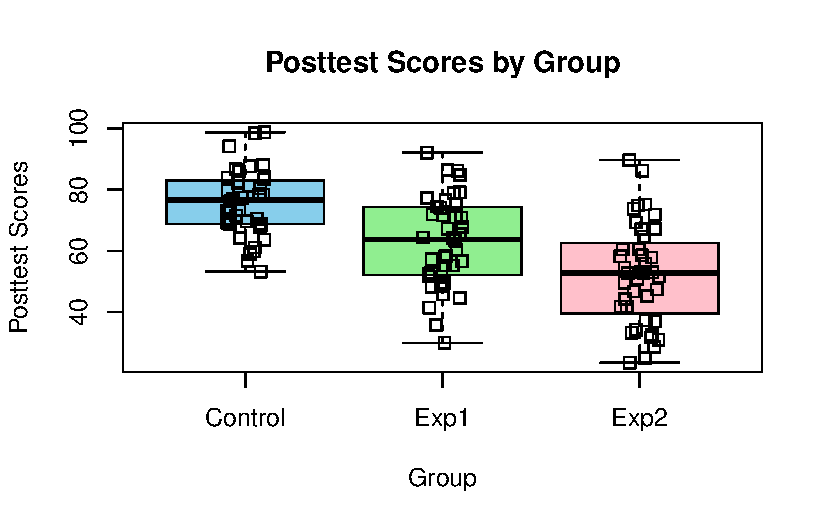
\includegraphics[keepaspectratio]{05_CRD_Intro_files/figure-pdf/fig-socialboxplot-1.pdf}}

}

\caption{\label{fig-socialboxplot}Boxplots of Post treatment scores by
group.}

\end{figure}%

The first line of code plots the boxplot and by inputting
\texttt{Posttest\textasciitilde{}Groups} as the first argument we are
say plot the values of \texttt{Posttest} by \texttt{Groups}. There are
extra graphical parameters specified to make the plot look a bit nicer.
The function \texttt{stripchart} is used to overlay the data points.
Based on these plots, there aren't any obvious outlying observations.

\subsection*{Equal population variance}\label{equal-population-variance}
\addcontentsline{toc}{subsection}{Equal population variance}

Since we only have sample data, we would not expect that the sample
variances to be exactly the same. If they are different it does not mean
the population variances are different. We expect them to differ a bit
due to chance simply because we are sampling from populations. Everytime
we sample from a population, the dataset will be different and so will
it's variability. The sample variances need to be similar enough so that
our assumption of equal population variance is reasonable. To check this
assumption, we can inspect the boxplots again and compare the heights.
More specifically, we look at the interquartile ranges (IQR). From
looking at the plot, the IQRs do not vary widely. If you prefer to look
at the actual values, we can use R to obtain them:

\begin{Shaded}
\begin{Highlighting}[]
\FunctionTok{sort}\NormalTok{(}\FunctionTok{tapply}\NormalTok{(multitask}\SpecialCharTok{$}\NormalTok{Posttest,multitask}\SpecialCharTok{$}\NormalTok{Group,IQR))}
\end{Highlighting}
\end{Shaded}

\begin{verbatim}
 Control     Exp2     Exp1 
14.01068 20.94529 21.97001 
\end{verbatim}

Another measure of variability we can look at, are the standard
deviations (sd's). With the same line of code but just replacing the
function we want to apply, we obtain the sd's of each group:

\begin{Shaded}
\begin{Highlighting}[]
\FunctionTok{sort}\NormalTok{(}\FunctionTok{tapply}\NormalTok{(multitask}\SpecialCharTok{$}\NormalTok{Posttest,multitask}\SpecialCharTok{$}\NormalTok{Group,sd))}
\end{Highlighting}
\end{Shaded}

\begin{verbatim}
 Control     Exp1     Exp2 
10.82887 14.60601 16.42678 
\end{verbatim}

The rule of thumb is to use the ratio of the smallest to largest
standard deviation and check whether it is smaller than five. In our
case, the smallest sd (of the Control group) is about 1.5 times smaller
than the largest sd (of the Exp 2 group) which is acceptable.

\subsection*{Normally distributed
errors}\label{normally-distributed-errors}
\addcontentsline{toc}{subsection}{Normally distributed errors}

We can check this assumption by looking at the residuals after model
fitting. A common misconception is to think that the response needs to
be normally distributed. However, it is only the unexplained variation,
i.e.~the errors or rasiduals, that we assume to be normally distributed.
of course, if the response has a clearly non-normal distribution
(e.g.~Binomial), then the residuals are likely to be non-normal as well.
So, we can check our response values before hand for obivous deviation
from normality, but we have to check this assumption again after fitting
our model. Things to look for are assymetric boxplots which indicate
skew distributions. We also want to check that the data points tend to
cluster around the median. In Figure~\ref{fig-socialboxplot}, there are
no signs of any clear deviation from normality. Other graphs we coudl
look at are histograms or Quantile-Quantile (Q-Q) plots. Q-Q plots show
the theoretical quantiles of the standard normal distribution against
the actual quantiles of our data. We want our data to be as close to the
xy line as possible (deviations in the tails are expected).

\begin{Shaded}
\begin{Highlighting}[]
\FunctionTok{qqnorm}\NormalTok{(multitask}\SpecialCharTok{$}\NormalTok{Posttest, }\AttributeTok{pty =} \DecValTok{4}\NormalTok{, }\AttributeTok{col =}\StringTok{"blue"}\NormalTok{)}
\FunctionTok{qqline}\NormalTok{(multitask}\SpecialCharTok{$}\NormalTok{Posttest, }\AttributeTok{col =} \StringTok{"red"}\NormalTok{)}
\end{Highlighting}
\end{Shaded}

\pandocbounded{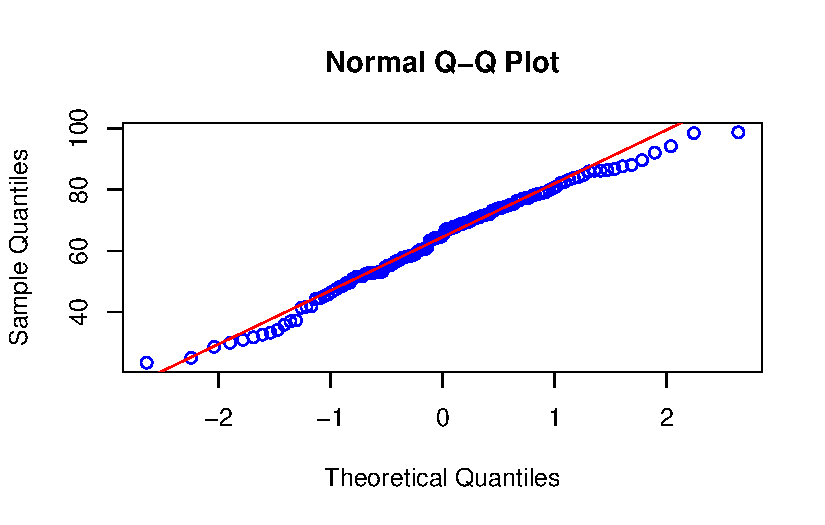
\includegraphics[keepaspectratio]{05_CRD_Intro_files/figure-pdf/qq-1.pdf}}

The \texttt{qqnorm} function plots the theoretical quantiles on the
x-axis and the sample quantile son the y-axis. So each point on the plot
corresponds to a quantile from the sample plooted against the expected
quantile from the standard normal distribution. As a reference we add a
straight 45-degree line (in red) using the \texttt{qqline} function to
indicate what perfect normality would look like.

\subsection*{Independent erros}\label{independent-erros}
\addcontentsline{toc}{subsection}{Independent erros}

In statistics, if one observation influences another in some way or
another, they are said to be dependent. For the type of data considered
here, there are two types of independence we require. Firstly,
observations within treatments should be independent and second,
observations between samples should be independent. Another way of
saying this, is \textbf{there should be independence within and among
treatments.} Depending on the direction of any violations, the within
treatment variance or among treatment variance can either be deflated or
inflated and treatment effects can be biased. This has considerable
impact on the test statistic (F-ratio for ANOVAs, more on this later)
which could lead to misleading results. \sidenote{\footnotesize Underwood (1996) has a
  very detailed explanation of the independence assumption (and the
  others) in the context of ANOVA. The book is for ecological
  experiments, but much of it pertains to all types of
  experiments.\linebreak\linebreak
\begin{CSLReferences}{2}{0}
\bibitem[\citeproctext]{ref-underwood_1996}
Underwood, A. J. 1996. {``Analysis of Variance.''} In \emph{Experiments
in Ecology: Their Logical Design and Interpretation Using Analysis of
Variance}, 140--97. Cambridge University Press.
\end{CSLReferences}
\linebreak}

Violations of independence typically occur when the experimental units
within or among treatments are connected in some way. Deependence within
a sample can occurs when they are taken in a non-random sequence. Doing
so typically allows some other variable to introduce dependence between
successive observations. For example, measurement drift (when a tool's
reading gradually changes over time), physical effects
(e.g.~temperature) of the location of experimental units or the
experimenter might become better (or worse) at taking the measurement as
they move along. If these variables are not taken into account (by
including them as factors in the model), it leads to a lack of
independence in the errors of our model. Specifically, they lead to
autocorrelated residuals; observations made closer together in time or
space are more similar to each other than expected.

An informal check we could do, is to plot the data in the order in which
they were collected (if this information is available) whether that is
temporally or spatially to see if any patterns emerge. To do this in R,
we can create a Cleveland dot plot.

\begin{Shaded}
\begin{Highlighting}[]
\FunctionTok{dotchart}\NormalTok{(multitask}\SpecialCharTok{$}\NormalTok{Posttest, }\AttributeTok{ylab =} \StringTok{"Order of observation"}\NormalTok{, }\AttributeTok{xlab =}\StringTok{"Post treatment test score"}\NormalTok{)}
\end{Highlighting}
\end{Shaded}

\pandocbounded{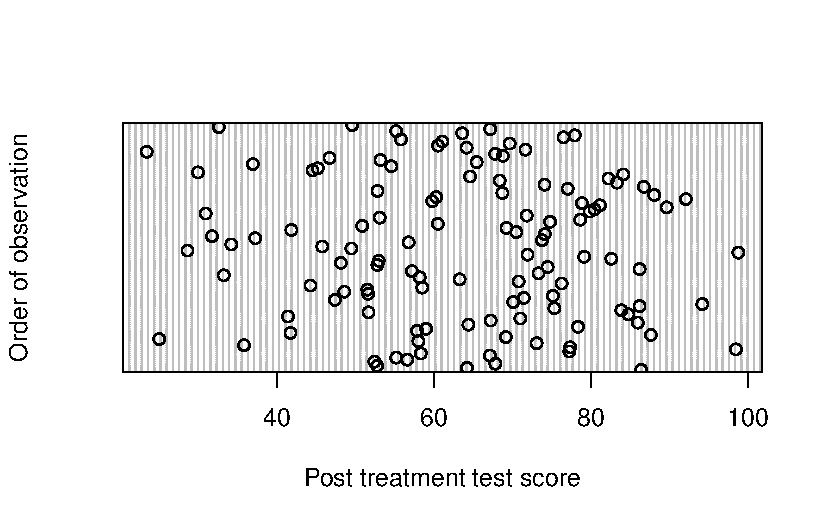
\includegraphics[keepaspectratio]{05_CRD_Intro_files/figure-pdf/unnamed-chunk-3-1.pdf}}

We have assumed that the order in which the observations appear in the
dataset are the order in which they were recorded. If there were any
factors that caused systematic trends, (i.e.~dependence) in the
observations, then there would be some kind of pattern in the dot chart.
For our example, there is no clear pattern. After fitting the model, we
can also plot the residuals against spatial coordinate or against order
to check for obvious patterns. This method, however, only detects
violations of independence if observations are related to time or space.

Dependence between treatments can occur if we apply the treatments to
the same group of experimental units or if experimental units from
different treatments are able to interact in some way during the
experiment. These types of violations including those mentioned above,
are ones that we can mostly prevent or control by properly designing the
experiment. When we control for factors that might induce dependence, we
can include them in our model.

Other reasons for dependence may not be as obvious or easy to eliminate
as we will see below. In the end, they may not have a strong impact on
our estimates but it is important to carefully scrutinise your design
and the system you are studying to identify possible sources of
dependence so that these can be either addressed and dealt with
properly.

In our example, within and among group dependence could be casued by the
students interacting or influencing each other in some way (by sharing
notes for example). During the lectures, this can be controlled by
careful monitoring and randomising their position in the lecture
theatre, but outside of lectures, it is less easy to control. Here we
can argue that if students interacted outside of lectures the impact on
their academic performance (as measured by the test) would likely be
neglibile. Here the integrity of the students is at play. It is not
really possible to diagnose this type of dependence after the fact, only
with careful design and implementation can these be avoided.

It is the onus of the experimenter to design and conduct experiments
that ensure independence. With more thought (and if we're lucky,
funding) all well-designed experiments should lead to independent data.
If violations are found after the fact, they cannot typically be
corrected and then methods that deal specifically with dependent data
(if appropriate) should be used\sidenote{\footnotesize A few of these methods are
  repeated measures ANOVA, mixed-models or hierarchical models.}.

\begin{tcolorbox}[enhanced jigsaw, colframe=quarto-callout-tip-color-frame, breakable, arc=.35mm, toptitle=1mm, colback=white, title=\textcolor{quarto-callout-tip-color}{\faLightbulb}\hspace{0.5em}{Note}, opacityback=0, bottomrule=.15mm, opacitybacktitle=0.6, colbacktitle=quarto-callout-tip-color!10!white, toprule=.15mm, rightrule=.15mm, bottomtitle=1mm, leftrule=.75mm, titlerule=0mm, coltitle=black, left=2mm]

In this course, you will always encounter data that has already been
collected and the description of the experiment will likely not be very
exhaustive. You might be task then with thinking about how the
assumption of independence could have been violated, but for the most
part we will assume the data are independent, both within and among
samples (unless otherwise stated).

\end{tcolorbox}

TIPS:

\begin{itemize}
\tightlist
\item
  increase focus, improve studying
\end{itemize}

\chapter{A Simple Model for a CRD}\label{a-simple-model-for-a-crd}

To analyse data collected from a Completely Randomised Design we could
use t-tests and compare the samples two at a time. This approach is
problematic for two reasons. Firstly, the test statistic of a t-test is
calculated with a standard deviation based only on the two samples it
considers and not the other samples collected in the experiment. We want
our test statistic to consider the variability in all samples. Second,
when we conduct multiple tests the overall Type 1 Error rate increases.
That is, when doing many tests, the chance of making \emph{at least one
wrong conclusion} increases with the number of tests (if you want to
know more see the box below). To avoid this, we will use the ANOVA
method which was specifically developed for comparing multiple means.

\begin{tcolorbox}[enhanced jigsaw, colframe=quarto-callout-caution-color-frame, breakable, arc=.35mm, toptitle=1mm, colback=white, title={Multiple Testing / Comparisons}, opacityback=0, bottomrule=.15mm, opacitybacktitle=0.6, colbacktitle=quarto-callout-caution-color!10!white, toprule=.15mm, rightrule=.15mm, bottomtitle=1mm, leftrule=.75mm, titlerule=0mm, coltitle=black, left=2mm]

When we conduct a test, there is always a possibility that a signficant
result is due to chance and not actually a real difference. In first
year, you were taught the Neyman-Pearson approach to hypothesis testing,
which entails setting a significance level (\(\alpha\)) for the test you
will conduct. This signficance level is the Type 1 error rate
(probability of falsely rejecting \(H_0\)). A common \(\alpha\) is 0.05,
meaning that 5\% of the time we will reject the null hypothesis even if
it is true. That means when we find a significant result, one of two
things have happened:

\begin{enumerate}
\def\labelenumi{\arabic{enumi}.}
\tightlist
\item
  Either we genuinely found a significant result or,
\item
  We were that unlucky, that our result is one of those 5\% cases.
\end{enumerate}

We will never know, this is the basis of statistical testing. We accept
that we cannot tell which of our conclusions are Type 1 Errors. When we
conduct many tests, the overall Type 1 Error rate increases. That is the
overall chance of \emph{at least one wrong conclusion} increases with
the number of tests conducted. This is not good! We already might be
wrong 5\% and we don't want to increase that risk even further when
conducting multiple tests.

\end{tcolorbox}

\section{The model}\label{the-model}

When we collect samples, we usually want to learn something about the
populations from which they were drawn. To do this, we can develop a
model for the observations that reflects the different sources of
variation believed to be at play.

For Completely Randomized Designs (CRDs), we have \(a\) samples with
population means \(\mu_1, \mu_2, \mu_3, \ldots, \mu_a\). A simple model
for each observation \(Y_{ij}\) is then given by:

\[
Y_{ij} = \mu_{i} + e_{ij},
\]

where

\[
\begin{aligned}
i & = 1, \dots, a \quad (a = \text{number of treatments}) \\
j & = 1, \dots, r \quad (r = \text{number of replicates}) \\
Y_{ij} & = \text{observation of the } j^{th} \text{ unit receiving treatment } i \\
\mu_i & = \text{mean of treatment } i \\
e_{ij} & = \text{random error with } e_{ij} \sim N(0, \sigma^2)
\end{aligned}
\]

That is, each observation is modeled as the sum of its population mean
and some random variation, \(e_{ij}\). This random variation represents
unexplained differences between individual observations, which we assume
to follow a normal distribution with mean 0 and constant variance across
all treatment groups. \sidenote{\footnotesize As opposed to non-constant variance
  across all treatment groups: \(e_{ij} \sim N(0, \sigma^2_{i})\) where
  the \(\sigma_i^2\)'s are different.}

We can change the notation slightly by arbitrarily dividing each mean
into a sum of two components: the overall mean \(\mu\) (the mean of the
entire dataset, which is the same as the mean of the \(a\)
means\sidenote{\footnotesize \(\mu = \frac{\sum\mu_i}{a}\)}) and the difference
between the population mean and the overall mean. In symbols, this
translates to:

\begin{equation}
\begin{aligned}
\mu_1 &= \mu + (\mu_1 - \mu) \\
\mu_2 &= \mu + (\mu_2 - \mu) \\
&\;\;\vdots \notag \\
\mu_a &= \mu + (\mu_a - \mu)
\end{aligned}
\end{equation}

The difference \((\mu_i - \mu)\) is the \textbf{effect of treatment}
\(i\), denoted by \(A_i\). So each population mean is the sum of the
overall mean and the part that we attribute to the particular treatment
(\(A_i\)):

\[
\mu_i = \mu + A_i, \quad i = 1, 2, \dots, a.,
\] where \(\sum A_i = 0\).

\begin{tcolorbox}[enhanced jigsaw, colframe=quarto-callout-caution-color-frame, breakable, arc=.35mm, toptitle=1mm, colback=white, title={Why the \(\sum A_i = 0\) constraint?}, opacityback=0, bottomrule=.15mm, opacitybacktitle=0.6, colbacktitle=quarto-callout-caution-color!10!white, toprule=.15mm, rightrule=.15mm, bottomtitle=1mm, leftrule=.75mm, titlerule=0mm, coltitle=black, left=2mm]

This constraint ensures that the treatment effects are expressed as
deviations from the overall mean. To see why this holds, take the sum of
both sides of the equation:

\[
\sum_{i=1}^{a} \mu_i = \sum_{i=1}^{a} (\mu + A_i).
\]

Expanding the right-hand side:

\[
\sum_{i=1}^{a} \mu_i = a\mu + \sum_{i=1}^{a} A_i.
\]

By definition, the overall mean \(\mu\) is the mean of the treatment
means:

\[
\mu = \frac{1}{a} \sum_{i=1}^{a} \mu_i.
\]

Multiplying both sides by \(a\) gives:

\[
\sum_{i=1}^{a} \mu_i = a\mu.
\]

Comparing this with our earlier equation:

\[
a\mu = a\mu + \sum_{i=1}^{a} A_i.
\]

Subtracting \(a\mu\) from both sides, we get:

\[
\sum_{i=1}^{a} A_i = 0.
\]

This constraint is a standard in ANOVA models to ensure that the
treatment effects are relative to the overall mean rather than being
arbitrarily defined. It is not an additional assumption; any \(a\) means
can be written in this way.

\end{tcolorbox}

Replacing \(\mu_i\) in the model above leads to the common
parameterization of a single-factor ANOVA model\sidenote{\footnotesize Often called
  \textbf{Model I}.}:

\[
Y_{ij} = \mu + A_{i} + e_{ij}
\]

where

\begin{equation}
\begin{aligned}
i & = 1, \dots, a \quad (a = \text{number of treatments}) \\
j & = 1, \dots, r \quad (r = \text{number of replicates}) \\
Y_{ij} & = \text{observation of the } j^{th} \text{ unit receiving treatment } i \\
\mu & = \text{overall or general mean} \\
A_i & = \text{effect of the } i^{th} \text{ level of treatment factor A} \\
e_{ij} & = \text{random error with } e_{ij} \sim N(0, \sigma^2)
\end{aligned}
\end{equation}

:::\{.callout-caution icon=``false'' collapse = ``false''\} \#\#
Comparison to regression

If you wanted to you could rewrite this with the regression notation
you've encounter before as a regression model with a single categorical
explanatory variables:

\[ Y_i = \beta_0 + \beta_1 T2_i + \beta_2 T3_i + e_i \]

where \(T2\) and \(T3\) are indicator variables (i.e.~\(T2 = 1\) if
observation \(i\) is from treatment 2 and 0 otherwise). The intercept
estimates the mean of the baseline category, here it is T1.

These two models are equivalent. The data are the exactly the same: in
both situations we have \(a\) groups and we are interested in the mean
response of these groups and the difference between them. The model
notation is just slightly different. In the ANOVA model we use \(\mu\)
and \(A_i\) instead of \(\beta_0\) and \(\beta_i\) which have different
meanings.

\begin{longtable}[]{@{}
  >{\centering\arraybackslash}p{(\linewidth - 2\tabcolsep) * \real{0.5000}}
  >{\centering\arraybackslash}p{(\linewidth - 2\tabcolsep) * \real{0.5000}}@{}}
\toprule\noalign{}
\begin{minipage}[b]{\linewidth}\centering
Regression
\end{minipage} & \begin{minipage}[b]{\linewidth}\centering
ANOVA
\end{minipage} \\
\midrule\noalign{}
\endhead
\bottomrule\noalign{}
\endlastfoot
\(\beta_0\) is the mean of the baseline category & \(\mu\) is the
overall mean \\
\(\beta_1\) is the difference between the means of category 2 and the
baseline category. & \(A_i\) is the effect of treatment \(i\),
i.e.~change in mean response relative to the overall mean. \\
\end{longtable}

When all the explanatory variables are categorical, which is mostly the
case in experimental data, it is more convenient to write the model in
the ANOVA form, for two reasons:

\begin{enumerate}
\def\labelenumi{\arabic{enumi}.}
\item
  The \(A_i\) notation is more concise, because we don't have to add all
  the dummy variables. This makes it easier to read and understand
  because there is only term per factor.
\item
  Mathematically it is more convenient. In this format all terms are
  deviations from a mean. This leads directly to sums of squares
  (squared deviations from a mean) and analysis of variance. We will see
  later that we can partition the total sum of squares into one part for
  every factor in the model. This allows us to investigate the
  variability in the response contributed by every model term (or
  factor).
\end{enumerate}

:::

The model can be interpreted as follows:

Each observation, \(Y_{ij}\), is the sum of the overall mean (\(\mu\)),
plus the effect of the treatment it belongs to (\(A_i\)), and some
random error (\(e_{ij}\)). We use two subscripts on the \(Y\). One to
identify the group (treatment) and the other to identify the subject
(experimental unit) within the group:

\begin{equation}
\begin{aligned}
Y_{1j} &= \mu + A_1 + e_{1j} \\ 
Y_{2j} &= \mu + A_2 + e_{2j} \\ 
Y_{3j} &= \mu + A_3 + e_{3j} \\

&\;\;\vdots \notag \\
Y_{aj} &= \mu +A_a + e_{aj} \\

\end{aligned}
\end{equation}

\section{Estimation}\label{estimation}

Okay, so we have a model which we need to \textbf{fit to our data}. When
we do this, we estimate the model parameters using our data. The
parameter we want to estimate are \(\mu\) (the overall mean), the
treatment effects (\(A_i\)) and \(\sigma^2\) (the error variance). As
for regression, we find \textbf{least square estimates} for the
parameters which minimize the residual or error sum of
squares\sidenote{\footnotesize error = observed - fitted.}:

\[ \text{SSE} = \sum_i\sum_je_{ij}^2 = \sum_i\sum_j (Y_{ij} - \hat{Y}_i)^2 = \sum_i\sum_j (Y_{ij} - \mu - A_i)^2\]
It turns out when we solve for the estimates that minimize the
SSE\sidenote{\footnotesize Another name for this is the residual sums of squares of
  RSS.}, we obtain the following estimators:

\[
\begin{aligned}
\hat{\mu} = \bar{Y}_{..} \\
\hat{\mu}_i = \bar{Y}_{i.}
\end{aligned}
\] and

\[\hat{A}_i =  \bar{Y}_{i.} - \bar{Y}_{..}\]

From linear model theory we know that the above are unbiased
estimates\sidenote{\footnotesize Unbiased means that the expected value of these
  statistics equal the parameter being estimated. In other words, the
  statistic equals the true parameter on average.} of \(\mu\) and the
\(A_i\)'s. What does this tell you? It tells you that we can use the
sample means as estimates for the true means. The estimated mean
response for treatment \(i\) is the observed sample mean of treatment
\(i\) and the observed overall mean is the estimated grand mean.

For the last parameter, the error variance, an unbiased estimator is
found by dividing the minimized SSE (i.e.~calculated with the least
square estimates) by its degrees of freedom:

\[ s^2 = \frac{1}{N-a}\sum_{ij}(Y_{ij} - \bar{Y}_{i.})^2 \]

This quantity is called the Mean Squares for Error (MSE) or residual
mean square. it has \((N-a)\) degrees of freedom since we have \(N\)
observations and have estimated \(a\) means. If you look at the formula
you'll notice that it is an average of the observed variance estimates
from the different treatment groups.

\begin{tcolorbox}[enhanced jigsaw, colframe=quarto-callout-caution-color-frame, breakable, arc=.35mm, toptitle=1mm, colback=white, title={Compare this with regression}, opacityback=0, bottomrule=.15mm, opacitybacktitle=0.6, colbacktitle=quarto-callout-caution-color!10!white, toprule=.15mm, rightrule=.15mm, bottomtitle=1mm, leftrule=.75mm, titlerule=0mm, coltitle=black, left=2mm]

Compare this with the equations you saw in the regression section.
Barring the extra subscript, the only difference is the equation for
calculating the fitted/predicted value.

In regression, the fitted value is:

\[ \hat{Y}_i = \hat{\beta}_0 + \hat{\beta}_1X_i \] and here it is:

\[ \hat{Y}_{ij} = \bar{Y}_{i.} = \hat{\mu} - \hat{A}_i \]

\end{tcolorbox}

\section{In context of the social media multitasking
example}\label{in-context-of-the-social-media-multitasking-example}

Let's take what we've learned so far and apply it to our example. We had
\(a = 3\) treatments each with \(r=40\) replicates. The model equation
is:

\[ Y_{ij} = \mu + A_{i} + e_{ij}  \]

where

\begin{equation}
\begin{aligned}
i & = 1, \dots, 3  \\
j & = 1, \dots, 40 \\
\end{aligned}
\end{equation}

If we write the model out for each treatment, we get:

\begin{equation}
\begin{aligned}
Y_{Cj} &= \mu + A_C + e_{Cj} \\ 
Y_{E1j} &= \mu + A_{E1} + e_{E1j} \\ 
Y_{E2j} &= \mu + A_{E2} + e_{E2j} \\
\end{aligned}
\end{equation}

and when we fit the model to the data, the predicted means for the
treatments are:

\begin{equation}
\begin{aligned}
\hat{Y}_{C} &= \hat{\mu} + \hat{A}_C = \bar{Y}_{C.}\\ 
\hat{Y}_{E1} &= \hat{\mu} + \hat{A}_{E1} = \bar{Y}_{E1.}\\ 
\hat{Y}_{E2} &= \hat{\mu} + \hat{A}_{E2} = \bar{Y}_{E2.}
\end{aligned}
\end{equation}

To fit this model in R, we use the \texttt{aov} function and then use
another function to extract the estimated parameters. By specifying type
= ``effects'', the function returns the \(\hat{A_i}\)'s

\begin{Shaded}
\begin{Highlighting}[]
\NormalTok{m1 }\OtherTok{\textless{}{-}} \FunctionTok{aov}\NormalTok{(Posttest}\SpecialCharTok{\textasciitilde{}}\NormalTok{Group, }\AttributeTok{data =}\NormalTok{ multitask)}

\FunctionTok{model.tables}\NormalTok{(m1, }\AttributeTok{type =} \StringTok{"effects"}\NormalTok{)}
\end{Highlighting}
\end{Shaded}

\begin{verbatim}
Tables of effects

 Group 
Group
Control    Exp1    Exp2 
 12.049  -0.703 -11.345 
\end{verbatim}

This tells us that the average score for students in the control group
is roughly 12\% higher than the overall average\sidenote{\footnotesize Remember:
  \(\mu_i = \mu + A_i\)}. Both experimental groups performed worse, with
students in the second group scoring, on average, about 11\% less than
the mean across all groups. We can also extract the overall mean and the
treatment means by specifying type = ``means'':

\begin{Shaded}
\begin{Highlighting}[]
\FunctionTok{model.tables}\NormalTok{(m1, }\AttributeTok{type =} \StringTok{"means"}\NormalTok{)}
\end{Highlighting}
\end{Shaded}

\begin{verbatim}
Tables of means
Grand mean
         
63.58527 

 Group 
Group
Control    Exp1    Exp2 
  75.63   62.88   52.24 
\end{verbatim}

The grand mean (i.e.~average of all test scores) was 64\% in this
experiment. The control group scored on average 76\% which is 12\%
higher than the overall mean and so on. So we have the estimates for the
effects, grand mean and treatment means.

The last paramter we need to estimate in the error variance
\(\sigma^2\). Have a look at the formula again:

\[ s^2 = \frac{1}{N-a}\sum_{ij}(Y_{ij} - \bar{Y}_{i.})^2 \]

If we focus on the sum and break into sums of squares for each treatment
\(i\), we get for the first treatment (let's say that is the control
group):

\[ \sum_{j}(Y_{1j} - \bar{Y}_{1.})^2 \] Which is the sum of the squared
differences between the observations in the control group and the mean
score of the group. We can easily calculated that in R assuming the
first treatment is the control group (there is no reason for this, we
just chose it)

\begin{Shaded}
\begin{Highlighting}[]
\NormalTok{control\_scores }\OtherTok{\textless{}{-}}\NormalTok{ multitask}\SpecialCharTok{$}\NormalTok{Posttest[multitask}\SpecialCharTok{$}\NormalTok{Group }\SpecialCharTok{==} \StringTok{"Control"}\NormalTok{] }\CommentTok{\# extract all scores for control group}
\NormalTok{mean\_control\_scores }\OtherTok{\textless{}{-}} \FunctionTok{mean}\NormalTok{(control\_scores) }\CommentTok{\# calculate bar Y\_1. {-} that is the mean score for control group}

\NormalTok{control\_sum\_squares }\OtherTok{\textless{}{-}} \FunctionTok{sum}\NormalTok{((control\_scores }\SpecialCharTok{{-}}\NormalTok{ mean\_control\_scores)}\SpecialCharTok{\^{}}\DecValTok{2}\NormalTok{) }\CommentTok{\# calculate sum of squares (not square of sum!)}
\end{Highlighting}
\end{Shaded}

First, we subset the dataset for the scores in the control group. Then
we find the mean and calculate the squared differences, whcih is all
summed together to give the sums of squares for treatment group 1. We
can repeat this for the remaining treatments and sum of the three sum of
squares together and divide by \(N-a\) to get the MSE.

\begin{Shaded}
\begin{Highlighting}[]
\CommentTok{\# Expermiment 1 }
\NormalTok{exp1\_scores }\OtherTok{\textless{}{-}}\NormalTok{ multitask}\SpecialCharTok{$}\NormalTok{Posttest[multitask}\SpecialCharTok{$}\NormalTok{Group }\SpecialCharTok{==} \StringTok{"Exp1"}\NormalTok{]}
\NormalTok{mean\_exp1\_scores }\OtherTok{\textless{}{-}} \FunctionTok{mean}\NormalTok{(exp1\_scores)}
\NormalTok{exp1\_sum\_squares }\OtherTok{\textless{}{-}} \FunctionTok{sum}\NormalTok{((exp1\_scores }\SpecialCharTok{{-}}\NormalTok{ mean\_exp1\_scores)}\SpecialCharTok{\^{}}\DecValTok{2}\NormalTok{)}

\CommentTok{\# Expermiment 2 }
\NormalTok{exp2\_scores }\OtherTok{\textless{}{-}}\NormalTok{ multitask}\SpecialCharTok{$}\NormalTok{Posttest[multitask}\SpecialCharTok{$}\NormalTok{Group }\SpecialCharTok{==} \StringTok{"Exp2"}\NormalTok{]}
\NormalTok{mean\_exp2\_scores }\OtherTok{\textless{}{-}} \FunctionTok{mean}\NormalTok{(exp2\_scores)}
\NormalTok{exp2\_sum\_squares }\OtherTok{\textless{}{-}} \FunctionTok{sum}\NormalTok{((exp2\_scores }\SpecialCharTok{{-}}\NormalTok{ mean\_exp2\_scores)}\SpecialCharTok{\^{}}\DecValTok{2}\NormalTok{)}

\CommentTok{\# Total sums of sqaures}
\NormalTok{sum\_squares }\OtherTok{\textless{}{-}} \FunctionTok{sum}\NormalTok{(control\_sum\_squares }\SpecialCharTok{+}\NormalTok{ exp1\_sum\_squares }\SpecialCharTok{+}\NormalTok{ exp2\_sum\_squares)}

\NormalTok{N }\OtherTok{\textless{}{-}} \FunctionTok{nrow}\NormalTok{(multitask) }\CommentTok{\# number of observations overall}
\NormalTok{a }\OtherTok{\textless{}{-}} \DecValTok{3} \CommentTok{\# number of treatment groups }


\NormalTok{sum\_squares}\SpecialCharTok{/}\NormalTok{(N}\SpecialCharTok{{-}}\NormalTok{a) }\CommentTok{\# MSE }
\end{Highlighting}
\end{Shaded}

\begin{verbatim}
[1] 200.1463
\end{verbatim}

Later we will see that we can extract this quantity easily from the
ANOVA table. But for now, this is a useful exercise to make sure you
understand the formula. So, \(\hat{\sigma^2} = s^2 = 200\) (rounded off
to the nearest integer) and \(\hat{\sigma} = s = 14\).

\section{Standard erros and confidence
intervals}\label{standard-erros-and-confidence-intervals}

In the previous section we saw how the parameters of the ANOVA model are
estimated. We also need a measure of uncertainty for each of these
estimates (in the form of a standard error, variance, or confidence
interval). Let's start with the variance for a treatment mean estimate:

\marginnote{\begin{footnotesize}

\textbf{Variance, Standard Deviation and Standard Error: what's all this
again?} The variance (Var) is a good way of measuring variability. The
Standard Deviation (SD) is the square root of the variance of a sample
or population. The Standard Error (SE) is the SD of an estimate.

\end{footnotesize}}

\[Var(\mu_i) = \frac{\sigma^2}{n_i} \]

Remember that the sampling distribution of the mean is
\(N(\mu,\frac{\sigma^2}{n})\) and here we assumed that the groups have
equal population variances.

If we assume that two treatment means are independent, the variance of
the difference between two means is:

\$\$

Var(\hat{\mu}\_i - \hat{\mu}\_j) = Var(\hat{\mu}\_i) + Var(\hat{\mu}\_j)
= \frac{\sigma^2}{n_i} + \frac{\sigma^2}{n_j}

\$\$ To estimate these variances we substitute the MSE for \(\sigma^2\)
as it is an unbiased estimate of the error variance (the variability
within each group).

\chapter{Analysis of Variance}\label{analysis-of-variance}

Although, I like the following description:

\begin{quote}
``Analysis of variance is better defined as a method of dividing
(analysing) a total variance into at least two components\ldots Using a
liberal definition of variances, analysis of variance can be said to
consist of estimating variances, and possibly of testing hypotheses
about them.''

--- Paul Seeger (1966)
\end{quote}

\chapter{Contrasts}\label{contrasts}

\part{Randomised Block Designs}

\part{Factorial Experiments}

\bookmarksetup{startatroot}

\chapter*{Glossary}\label{glossary}
\addcontentsline{toc}{chapter}{Glossary}

\markboth{Glossary}{Glossary}

\begin{description}
\item[\phantomsection\label{glossary-experimental-design}{Experimental
Design}]
A systematic method to plan experiments in a way that ensures valid and
unbiased results.
\item[\phantomsection\label{glossary-anova-analysis-of-variance}{ANOVA
(Analysis of Variance)}]
A statistical method used to compare the means of three or more groups
to determine if at least one differs significantly.
\item[\phantomsection\label{glossary-replication}{Replication}]
When treatments are applied to more than one experimental unit. The
number of experimental units per treatment is the number of replicates
an experiment has.
\item[\phantomsection\label{glossary-randomization}{Randomization}]
A process of randomly assigning subjects or experimental units to
treatments.
\item[\phantomsection\label{glossary-blocking}{Blocking}]
A technique to account for variability by grouping similar experimental
units.
\item[\phantomsection\label{glossary-factor}{Treatment Factor}]
An independent variable in an experiment.
\item[\phantomsection\label{glossary-level}{Treatment Level}]
The specific values or categories of a factor.
\end{description}

{[}Treatments{]}





\end{document}
